%\ce{BrO}  Evaluation and its limitations
This chapter discusses the evaluation of the \ce{BrO} Column densities, calculated from the spectra recorded by the spectroscopic instruments of NOVAC. The quality of the BrO retrieval hereby is defined by the BrO retrieval error.\\
\Cref{fig:allbroerrordistribution} shows the BrO "Multi Add" retrieval error distribution, which is centered around $1.1e^{13}$ to $1.4e^{13}$. The instruments of Nevado del Ruiz are coloured blue, while the the instruments of Tungurahua are coloured in yellow to red.\\
\\
The evaluation of the data from NOVAC are parted into the evaluation of \ce{SO2} and the evaluation of BrO. While the retrieving of \ce{SO2} is relatively easy due to the high amount of \ce{SO2} in the plume (magnitude of \ce{SO2} at Tungurahua $\approx 1e^{18}$), the \ce{BrO} evaluation is much more problematic (as it can be seen in \Cref{fig:plumeref}). The magnitude of \ce{BrO} SCD is around $\approx 1e^{14}$. \\
%
\begin{figure}
	\subfigure{
	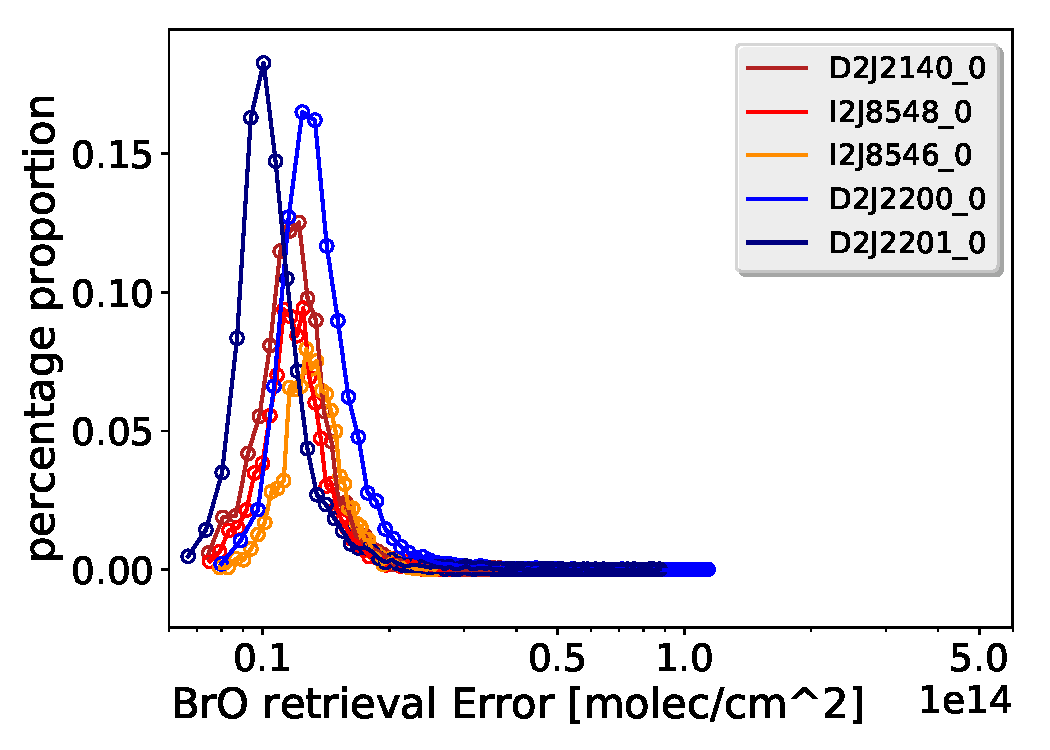
\includegraphics[width=0.49\linewidth]{E:/Masterarbeit/BrO_Error_Distribution/sametimeBrOErrorDistribution}}
\subfigure{
	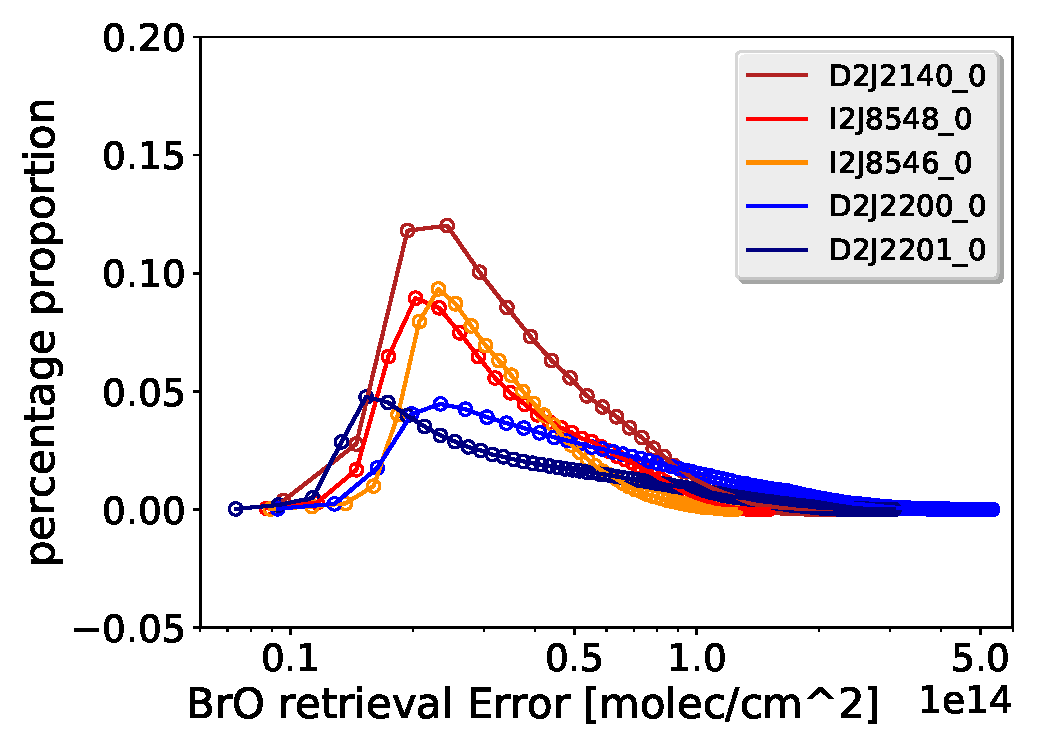
\includegraphics[width=0.49\linewidth]{E:/Masterarbeit/BrO_Error_Distribution/AllBrOErrorDistribution}}
	\caption{\ce{BrO} error distribution shown for all instruments considered in this thesis. The left plot shows the \ce{BrO} distribution for the "same time retrieval", the left plot shows the \ce{BrO} error distribution for the evaluation with a reference from another time, where the temporal difference between plume and reference is not longer that two weeks. 
	The peaks for the single instrument are located at: D2J2140: 1.2e+13;
		 I2J8548: 1.3e+13$\frac{molec}{cm^2}$;
		I2J8546: 1.4e+13$\frac{molec}{cm^2}$;
		D2J2200: 1.4e+13$\frac{molec}{cm^2}$;
		D2J2201: 1.1e+13$\frac{molec}{cm^2}$}
	\label{fig:allbroerrordistribution}
\end{figure}
%
This results in a larger uncertainty of the \ce{BrO}  SCD. Most of the \ce{BrO} data (98.3\% of the data) are below the detection limit of \ce{BrO}$_{err}$/\ce{BrO}$_{value}$<1/4. In comparison SCD's of \ce{SO2} in almost all cases (99.5\% of the data)  are above the detection limit. \\
%
Choosing a different reference than the reference measured at the same time as the plume in 99\% of the cases results in an increasing of the absolute error. 
Thus a \ce{BrO} error which is smaller than the "Same Time Error" is often not  possible to retrieve. 
However, for a contaminated same-time-reference the relative error might decrease due to the underestimation of the gas amount. \\
Due to the large uncertainty of \ce{BrO} relative to \ce{SO2} the optimization of the \ce{BrO} error is of particular importance. Therefore, the reference is chosen with respect to the \ce{BrO} error to maximize the quality of the \ce{BrO}/\ce{SO2} ratio. \\
\\
The amount of gas free alternative references is around 1500 per year. To make an optimal choice, it is necessary to examine the conditions which influence the \ce{BrO} retrieval.\\
Every spectrum is measured under certain conditions. These measuring conditions generally are not equal for the plume and the reference. References for which the surrounding conditions e.g temperature or cloudiness are equivalent with the surrounding conditions of the  plume measuring lead to a small error.\\
In the following, we take a closer look at the dependence of the \ce{BrO} error on external parameters. 
%
\subsubsection*{Data used for the analysis}
For this analysis, every plume reference pair of the observed time span is used. Thus 1000 recorded "multi add" spectra result in $1000^2$ possible plume reference pairs and the corresponding differences in the external parameter and their associated \ce{BrO} error.


\section{\ce{BrO} error dependence on external parameters \label{Chap:BROErr}}
The measurement and evaluation of the spectra monitored with NOVAC depends on the surrounding conditions like temperature or cloudiness \citep{lubcke2014optical}\\
Thus, the surrounding conditions need to be taken into account for choosing a new reference.\\
The better the surrounding conditions for the reference coincide with the conditions for the plume measurement, the lower is the \ce{BrO} error. \\
	\\
The surrounding conditions that are considered in this thesis are: 
	\begin{itemize}
		\item Temporal difference between measuring the plume and the reference.
		\item Temperature, 
		\item Colorindex, 
		\item Exposure time, 
		\item Elevation angle, 
		\item Daytime 	
	\end{itemize}
The analysis of these external parameters are performed for spectra recorded at Tungurahua and Nevado del Ruiz. At Tungurahua three instruments with data recorded in the time span from July in 2008 to August in 2009 are used. Nevado del Ruiz contributes with two instruments in the time from the end of 2009 to the end of 2011.
%	
\subsection{Temporal difference}
%
\begin{figure}
	\centering
	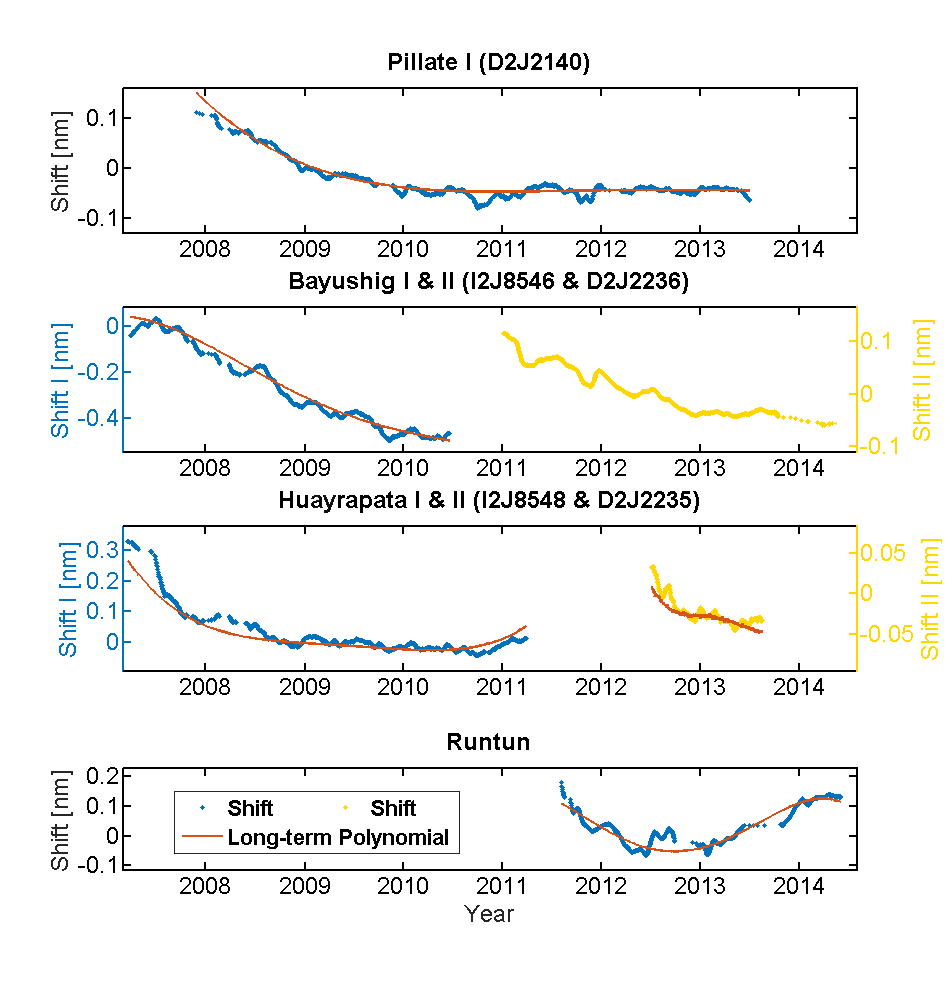
\includegraphics[width=1\linewidth]{Bilder/Simon/Bilder_Tung/Drift_Komplett_NEW}
	\caption{Wavelength shift over the time. The shift is shown for six NOVAC- instruments from Tungurahua. The red and yellow dots show the running mean over 20 days. Red line indicates a temperature independent long term polynomial. Source: \cite{WarnachSimon}}
	\label{fig:driftkomplettnew}
\end{figure}
%
\begin{figure}
	\subfigure[]{
		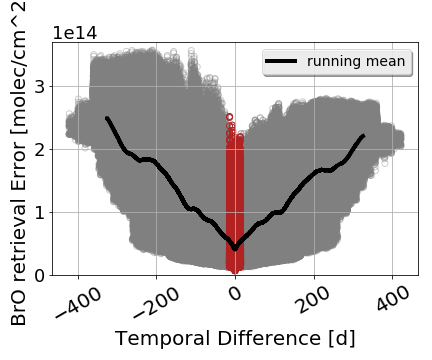
\includegraphics[width=0.5\linewidth]{Bilder/Datum}}
	\subfigure[]{
		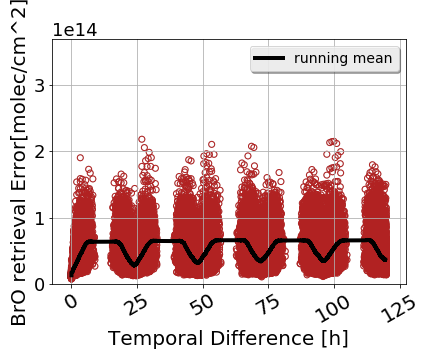
\includegraphics[width=0.5\linewidth]{Bilder/datumkurz}}	
	\caption{The \ce{BrO} error as a function of the temporal difference shown for the Pillate instrument from Tungurahua (2008-2009). (a) Temporal differences up to 400 days. (b) Temporal differences up to 120h. The periodical \ce{BrO}  error evolution indicates the impact of the daytime}
	\label{fig:dat}
\end{figure}
%
Due to instrument drifts the fit quality decreases with the time difference between recording the plume and the reference. This could be a result of a wavelength shift over time observed by \citet{WarnachSimon}. As a result of the observed wavelength shift, the instrument function of the plume, does not match with the instrument function of the reference, thus the retrieving errors increase. \citet{WarnachSimon} suggests that the drift is caused by a hysteresis effect. \Cref{fig:driftkomplettnew} shows the wavelength shift as a function of the time for six NOVAC instruments located at Tungurahua in the time between 2008 to 2014. In this thesis for the analysis data of Tungurahua between 2008 to the mid of 2009 are used. \Cref{fig:driftkomplettnew} shows a rather steep drift in this time interval. \citet{WarnachSimon} observed a decrease of the shift after initial negative drift after the first two years at Pillate. Thus, it is observed that the temporal difference becomes less important for old instruments.\\
When using reference and plume spectra of the same time, these effects are cut out since the shift is equal for the plume and reference spectrum.
For an increasing temporal different between reference and plume measurement time the fit quality decreases and so does the \ce{BrO} error.\\
To examine the effect of the temporal difference on the retrieved \ce{BrO} error, for all reference-plume pairs the corresponding \ce{BrO} error is calculated. Due to the large amount of reference plume pairs within one year, it takes more than a month (Hardware details: Intel(R) Core(TM) i5-4570 CPU @ 3.20Ghz 64 Bit operating system, amount of kernels: 4) to evaluate the corresponding \ce{BrO} error for every possible reference-plume pair of one instrument. We did this for the  D2J2140 instrument installed at Tungurahua:\\
In \Cref{fig:dat} the \ce{BrO} error as a function of the time difference between recording the plume and the reference is shown. The running mean is plotted with a black line. \\
In \Cref{fig:dat} (a) it can be seen that a large temporal difference results in an increase of the \ce{BrO}  error of up to 600\%. \ce{BrO} errors of such magnitudes are too large for our purposes. Therefore, it is useful to set a maximal temporal difference, to prevent too large \ce{BrO} error and to reduce the calculation time.
%
In \Cref{fig:dat} (a) it can be seen that the evolution of the \ce{BrO}  error with the temporal difference is symmetric around zero. Thus it is not necessary to distinguish between positive or negative temporal differences.
%
\Cref{fig:dat} (b) shows the evolution of the \ce{BrO} error for a maximal absolute temporal difference of 120 hours. It is only possible to record data during daytime. This causes the lack of data in the night time. A periodic decrease of the \ce{BrO} error can be seen. This is a result of a decrease of the \ce{BrO} error when the surrounding conditions coincidence. In this case the daytime coincidence causes the \ce{BrO}  error decrease. This effect is analysed in detail in \Cref{chap:daytime}.\\

The maximal temporal difference should be large enough to ensure a sufficient amount of references to be able to pick a reference with similar conditions. However, the maximal temporal difference should be small enough to prevent too large \ce{BrO} errors due to long term shifts.\\
\\
To evaluate the maximal time difference, for which we still get reliable results for every plume, where the "same time reference" is contaminated, the alternative reference is chosen, which leads to the minimal \ce{BrO} error.\\
%
In \Cref{fig:Hist} a histogram with the probability of picking the best reference as a function of the time difference is plotted. Obviously, the best results are achieved, if the day of measuring the plume is the same day as measuring the reference. A Gaussian fit is used to fit the data of the histogram We allow all time differences within two sigma area. Thus, the maximal time difference is 14 days\\
% histogram
\begin{figure}
	\centering
	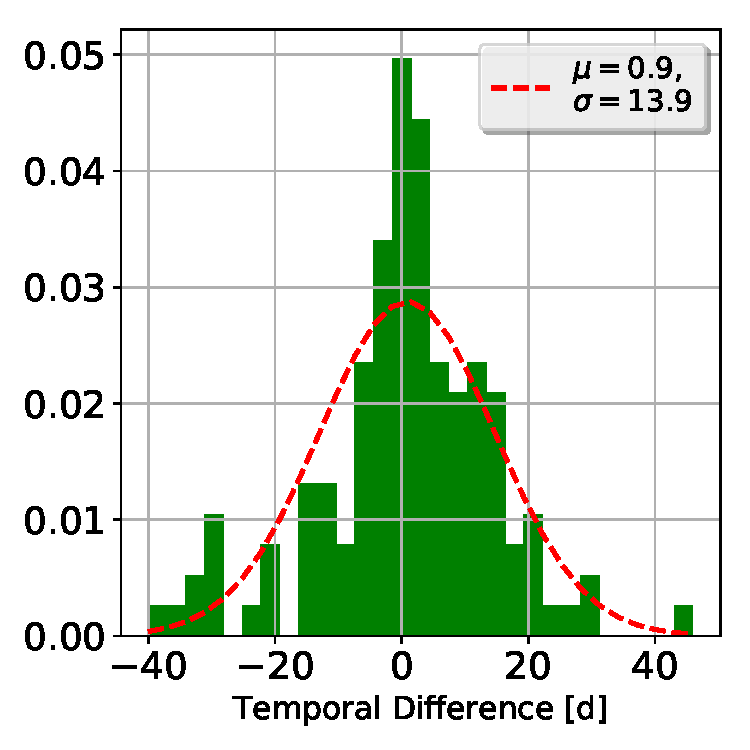
\includegraphics[width=0.7\linewidth]{Bilder/Hist}
	\caption{Histogram showing the frequency of getting the best reference as function of the temporal difference between plume and reference measuring. A Gaussian-like distribution is retrieved. The red dotted line visualizes a Gaussian fit for the shown histogram.}
	\label{fig:Hist}
\end{figure}
% remaining possible reference spectra
\begin{table}[h]
	\centering
	\begin{tabular}{|p{1.8cm}|p{2.15cm}|p{2.15cm}|p{2.15cm}|p{2.15cm}|p{2.15cm}|}
		%	\toprule
		Instrument	&D2J2140&I2J8546& I2J8548&D2J2200&D2J2201\\
		\toprule
		Mean&84.6 &163.7 &217.1&284.0 &225.6 \\
		\midrule
		Std&
		35.8&% $\equiv$ 100\%&
		29.9&% $\equiv$ 100\%&
		64.8&% $\equiv$ 100\%&
		69.5&% $\equiv$ 100\%&
		41.2\\% $\equiv$ 100\%\\
		\midrule
		Min&
		8 &%$\equiv$ 100\%&
		113&% $\equiv$ 100\%&
		97 &%$\equiv$ 100\%&
		64&% $\equiv$ 100\% &
		63\\% $\equiv$ 100\%\\
		\midrule
		Max&
		169&% $\equiv$ 100\%&
		214&% $\equiv$ 100\%
		399&% $\equiv$ 100\%
		433&%  $\equiv$ 100\%
		297\\% $\equiv$ 100\% \\
		\bottomrule
	\end{tabular}
	\caption{Amount of possible references when restricting the time span between plume and reference to two weeks. Here in the ”Mean” and “Std” row for each  instrument the average restriction is shown with the corresponding standard deviation. The “Min” and “Max” rows show the extend of restriction in the extreme cases (minimum and maximum amount of available references / restriction ratio).}
	\label{Tab:refstime}
\end{table}	
By restricting the temporal difference to 14 days, the amount of possible gas free references decreases to an average of 195 alternative references per contaminated plume (see \cref{Tab:refstime}). Hereby every plume has potential alternative reference spectra. The minimum amount of references is 8.\\
If a continuously evaluation is required, this means the spectra are evaluated directly after the recording, the number of suitable gas free references halves since only references recorded before the plume are available.\\
\nopagebreak
For the following analysis of the remaining external parameters all temporal differences are below 14 days.
\begin{figure}
	\centering
	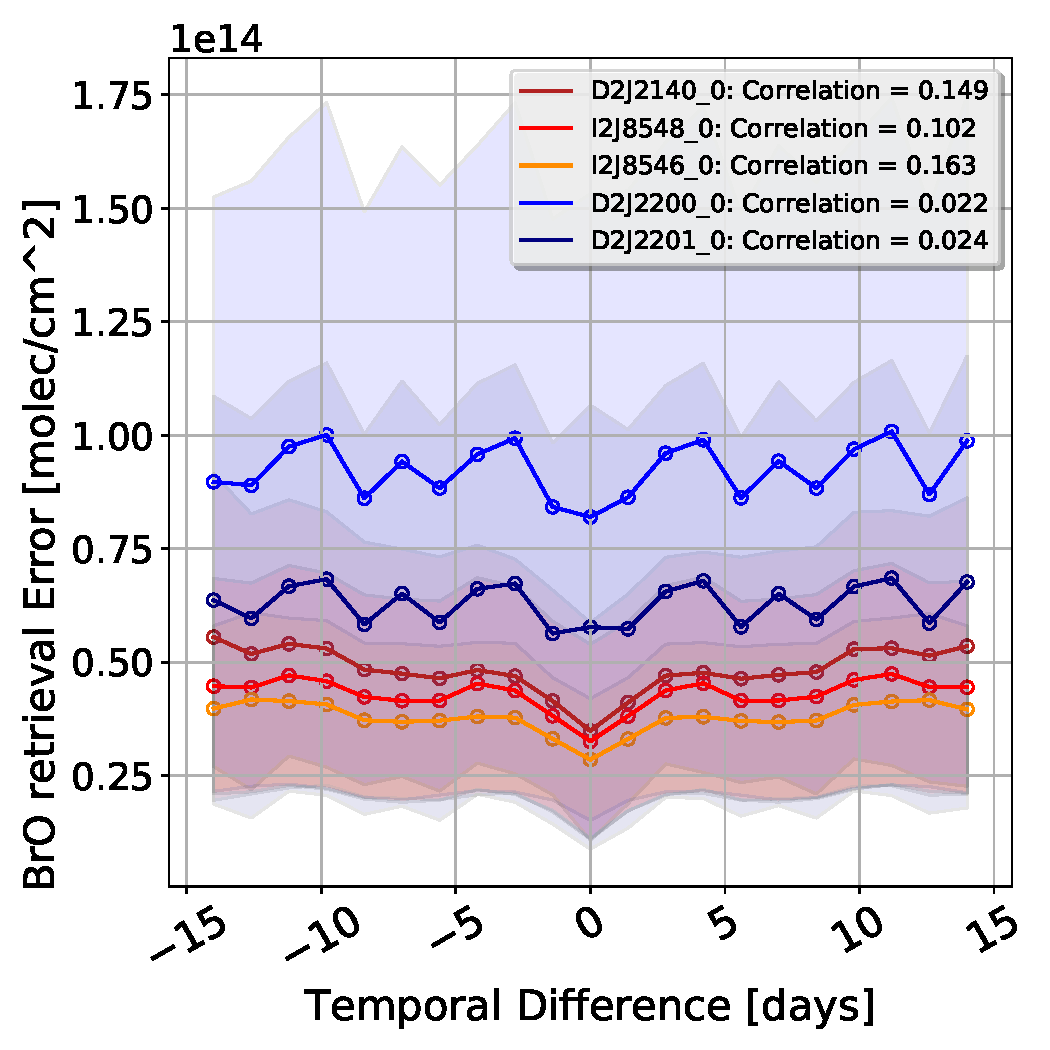
\includegraphics[width=0.7\linewidth]{Bilder/DatallInstruments}
	\caption{The \ce{BrO} measurement error as a function of the temporal difference in days between the reference and the plume is shown for each of the individual instruments at Tungurahua and Nevado del Ruiz. The instruments at Nevado del Ruiz are coloured in blue, while the instruments at Tungurahua are coloured in red colour tones.  To evaluate the plume spectra all reference spectra with a temporal distance of no longer than two weeks are used. An increase of the \ce{BrO} error with the absolute difference in temperature is observable. This is quantified by a correlation between the \ce{BrO} retrieval error and the absolute temporal difference. The plots reveal a symmetry around the axis with zero temperature difference.}
	\label{fig:datallinstruments}
\end{figure}


\subsection{Temperature}
% fig_curves CAPTION
\begin{figure}
	\centering
	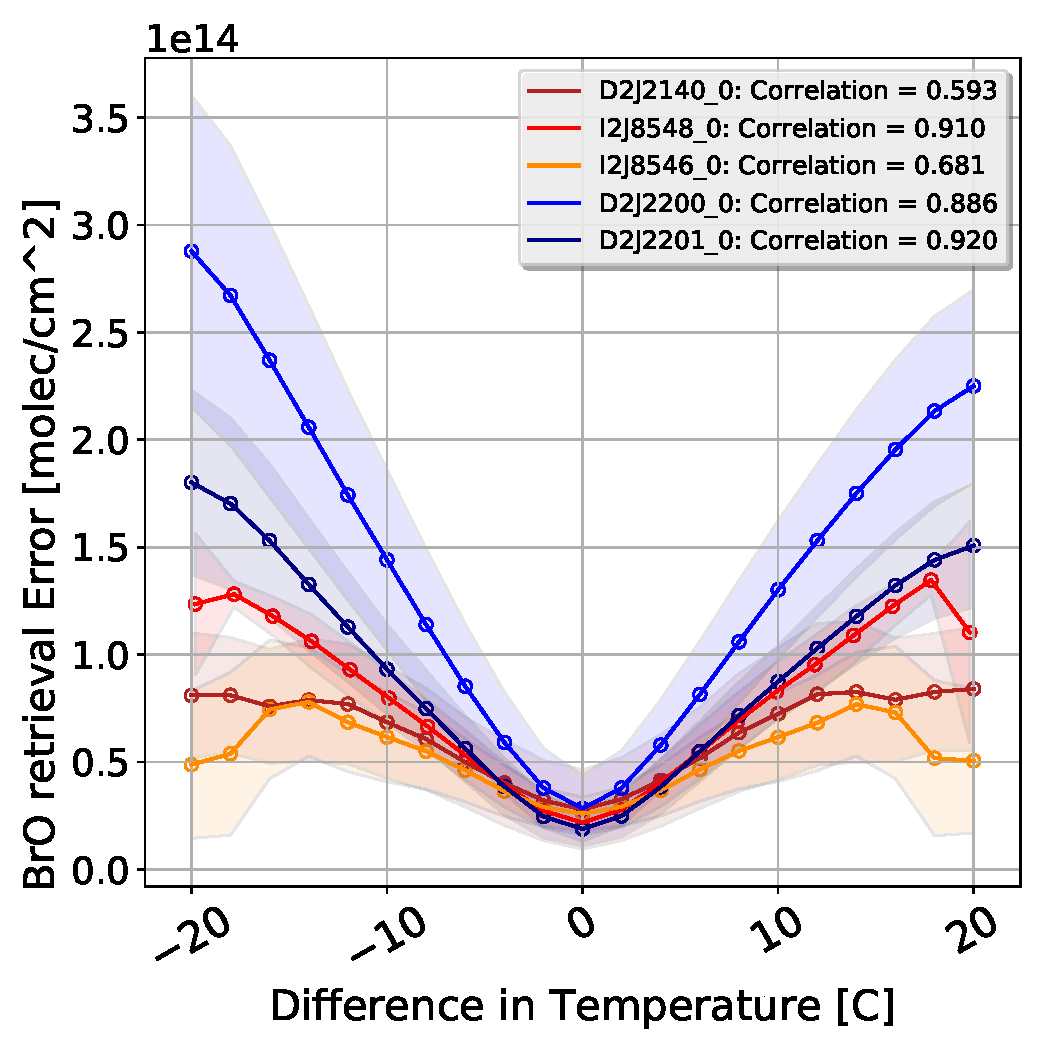
\includegraphics[width=0.7\linewidth]{Bilder/DiffTempallInstruments}
	\caption{The \ce{BrO} measurement error as a function of the difference of temperature between the reference and the plume is shown for each of the individual instruments at Tungurahua and Nevado del Ruiz. To evaluate the plume spectra all reference spectra with a temporal distance of no longer than two weeks are used. An increase of the \ce{BrO} error with the absolute difference in temperature is observable. This is quantified by a correlation between the \ce{BrO} retrieval error and the absolute difference in temperature. The plots reveal a symmetry around the axis with zero temperature difference.}
	\label{fig:difftemp}
\end{figure}
% individual text
The instrument design of the NOVAC instruments compromises between accuracy and robustness as explained in \Cref{NOVAC}. In particular, there are no internal thermal stabilizations installed as an attempt to reduce the instruments power consumption. This can influence the recorded spectra.\\	
Each pixel of the spectrometer, which is used for the DOAS experiment, collects photons of a certain wavelength range.\\
The calibration for the wavelength to pixel mapping (WMP) is commonly done with a mercury lamp or by the comparison with the high defined Kuruz spectrum.
As the WMP depends on the optical alignment of the spectrometer, which itself depends on the temperature, it is not constant.
Changes in the spectrometers temperature can cause changes in the instrument line function and shifts in the WMP (\citep{pinardi2007influence}). 
% short term wavelength
\begin{figure}		
	\subfigure[]{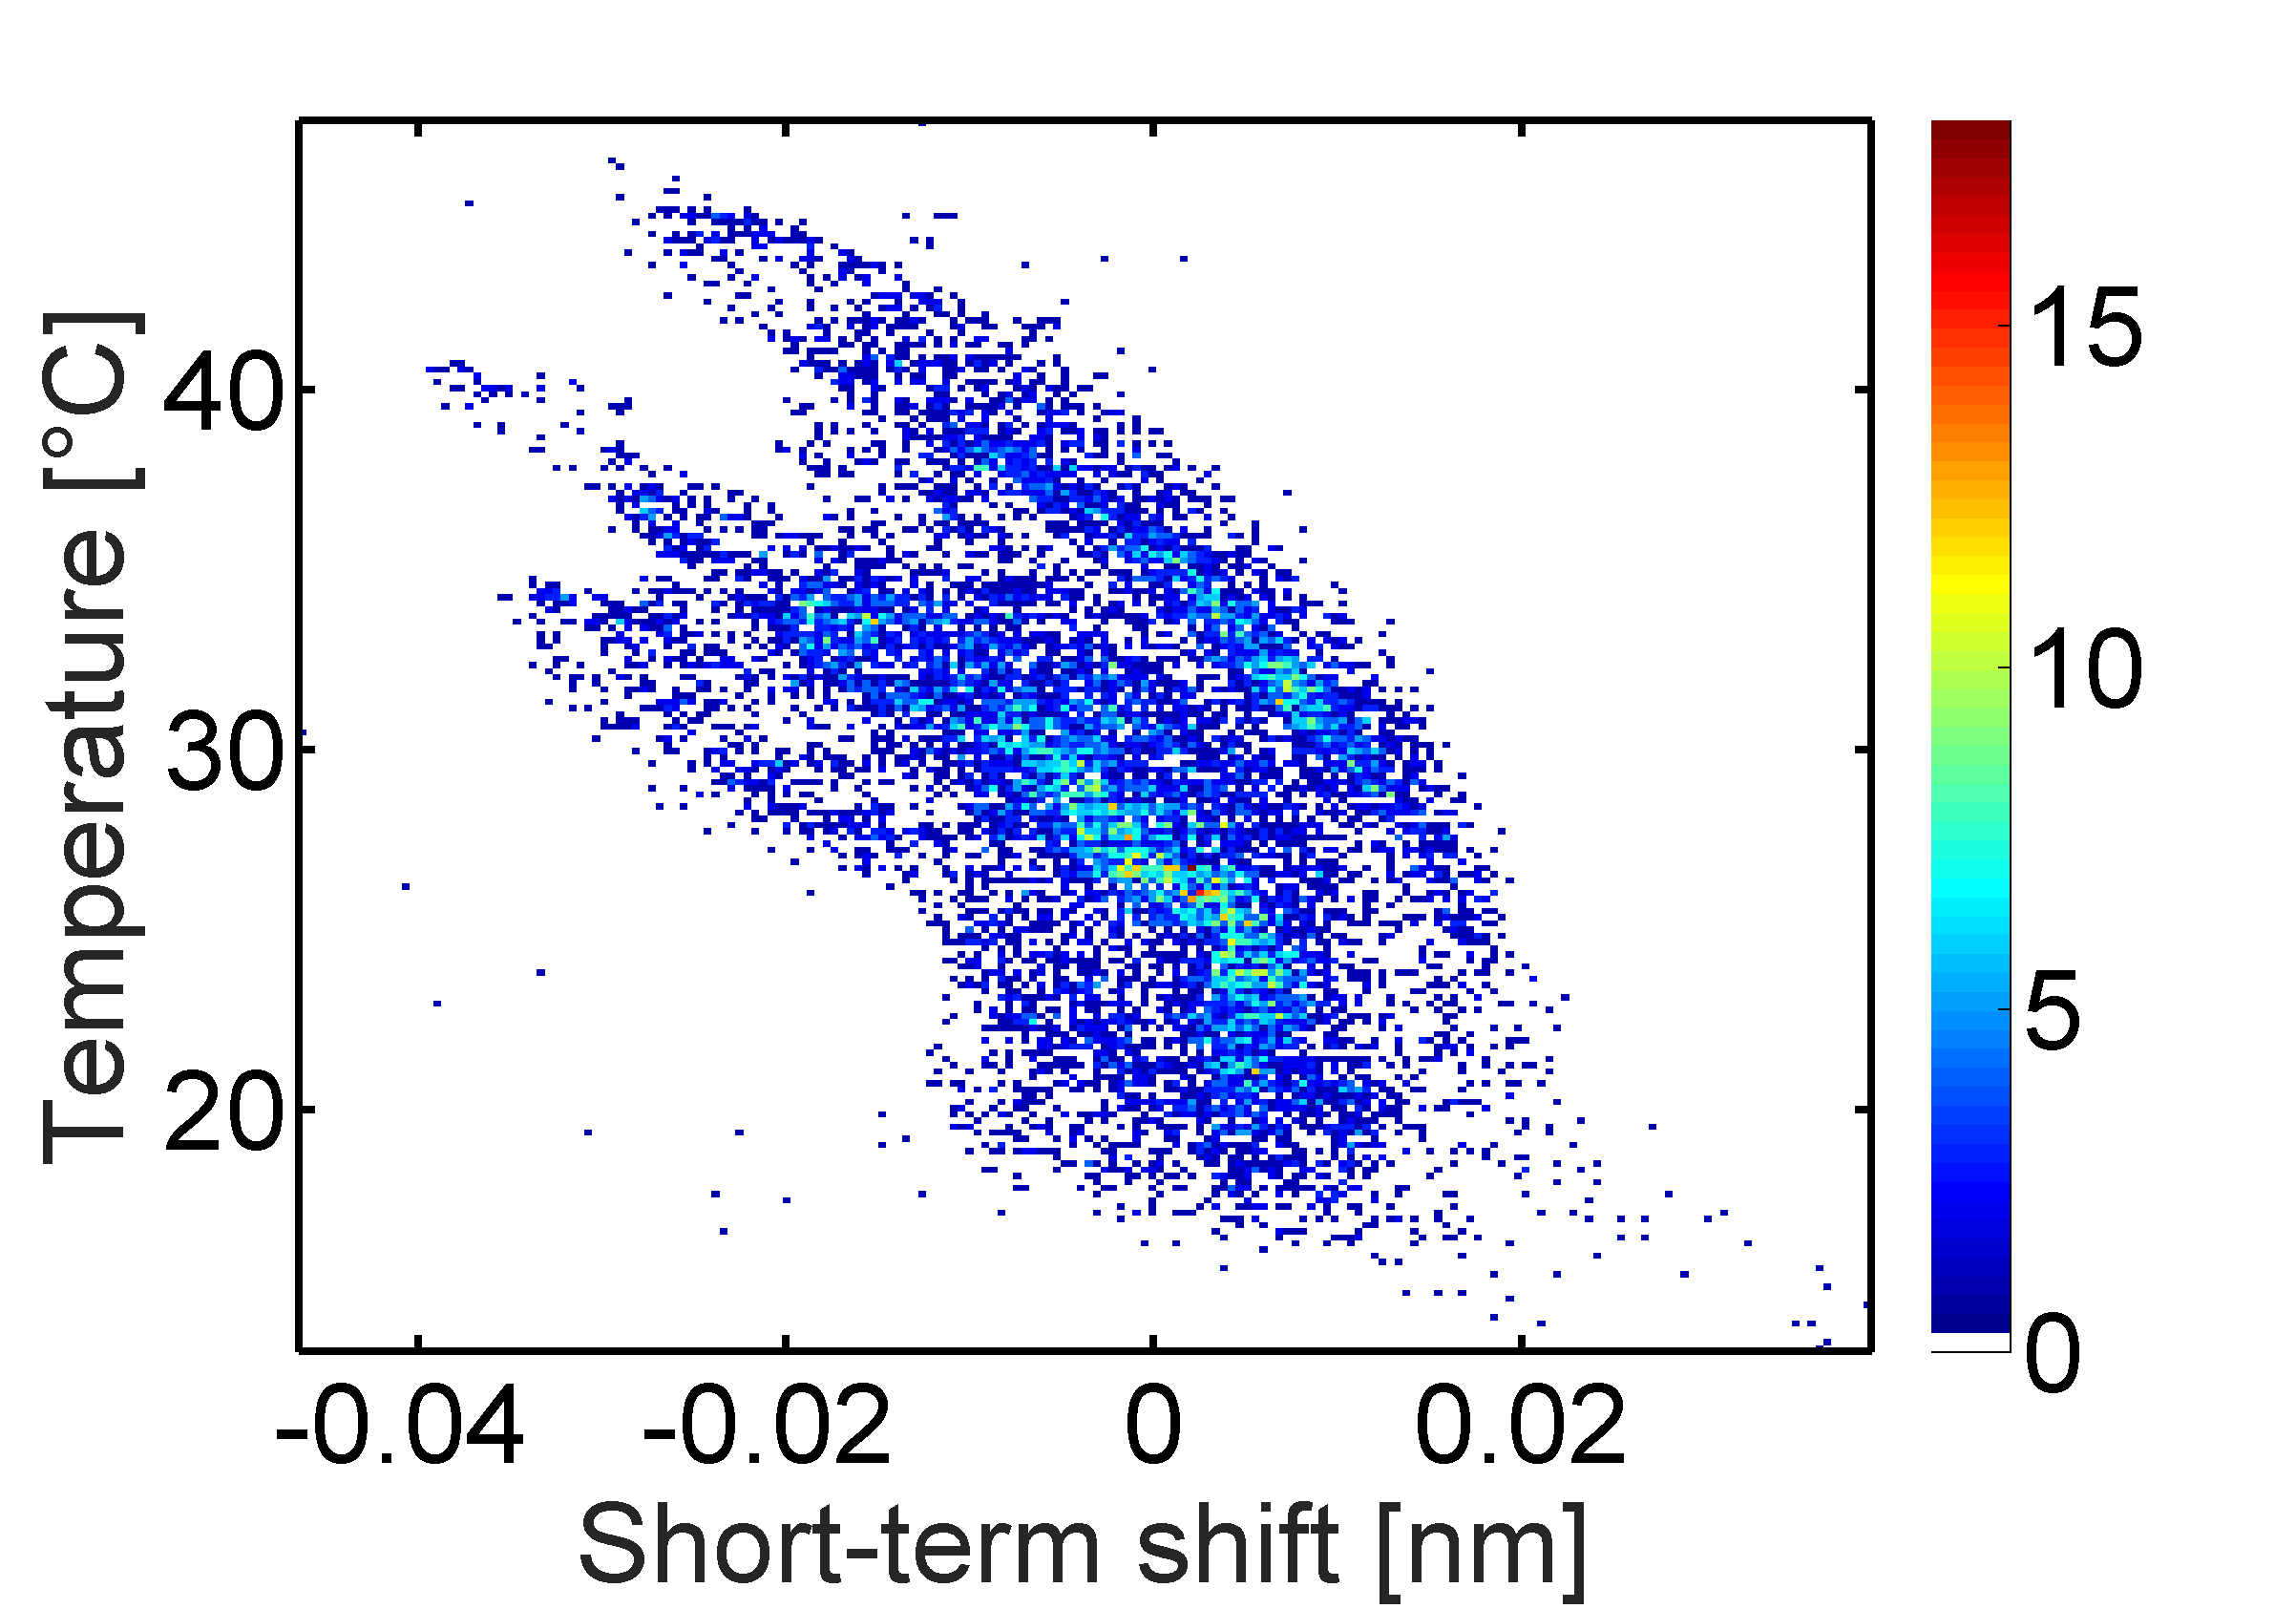
\includegraphics[width=0.49\textwidth]{Bilder/Simon/Bilder_Tung/D2J2140_Before}}
	\subfigure[]{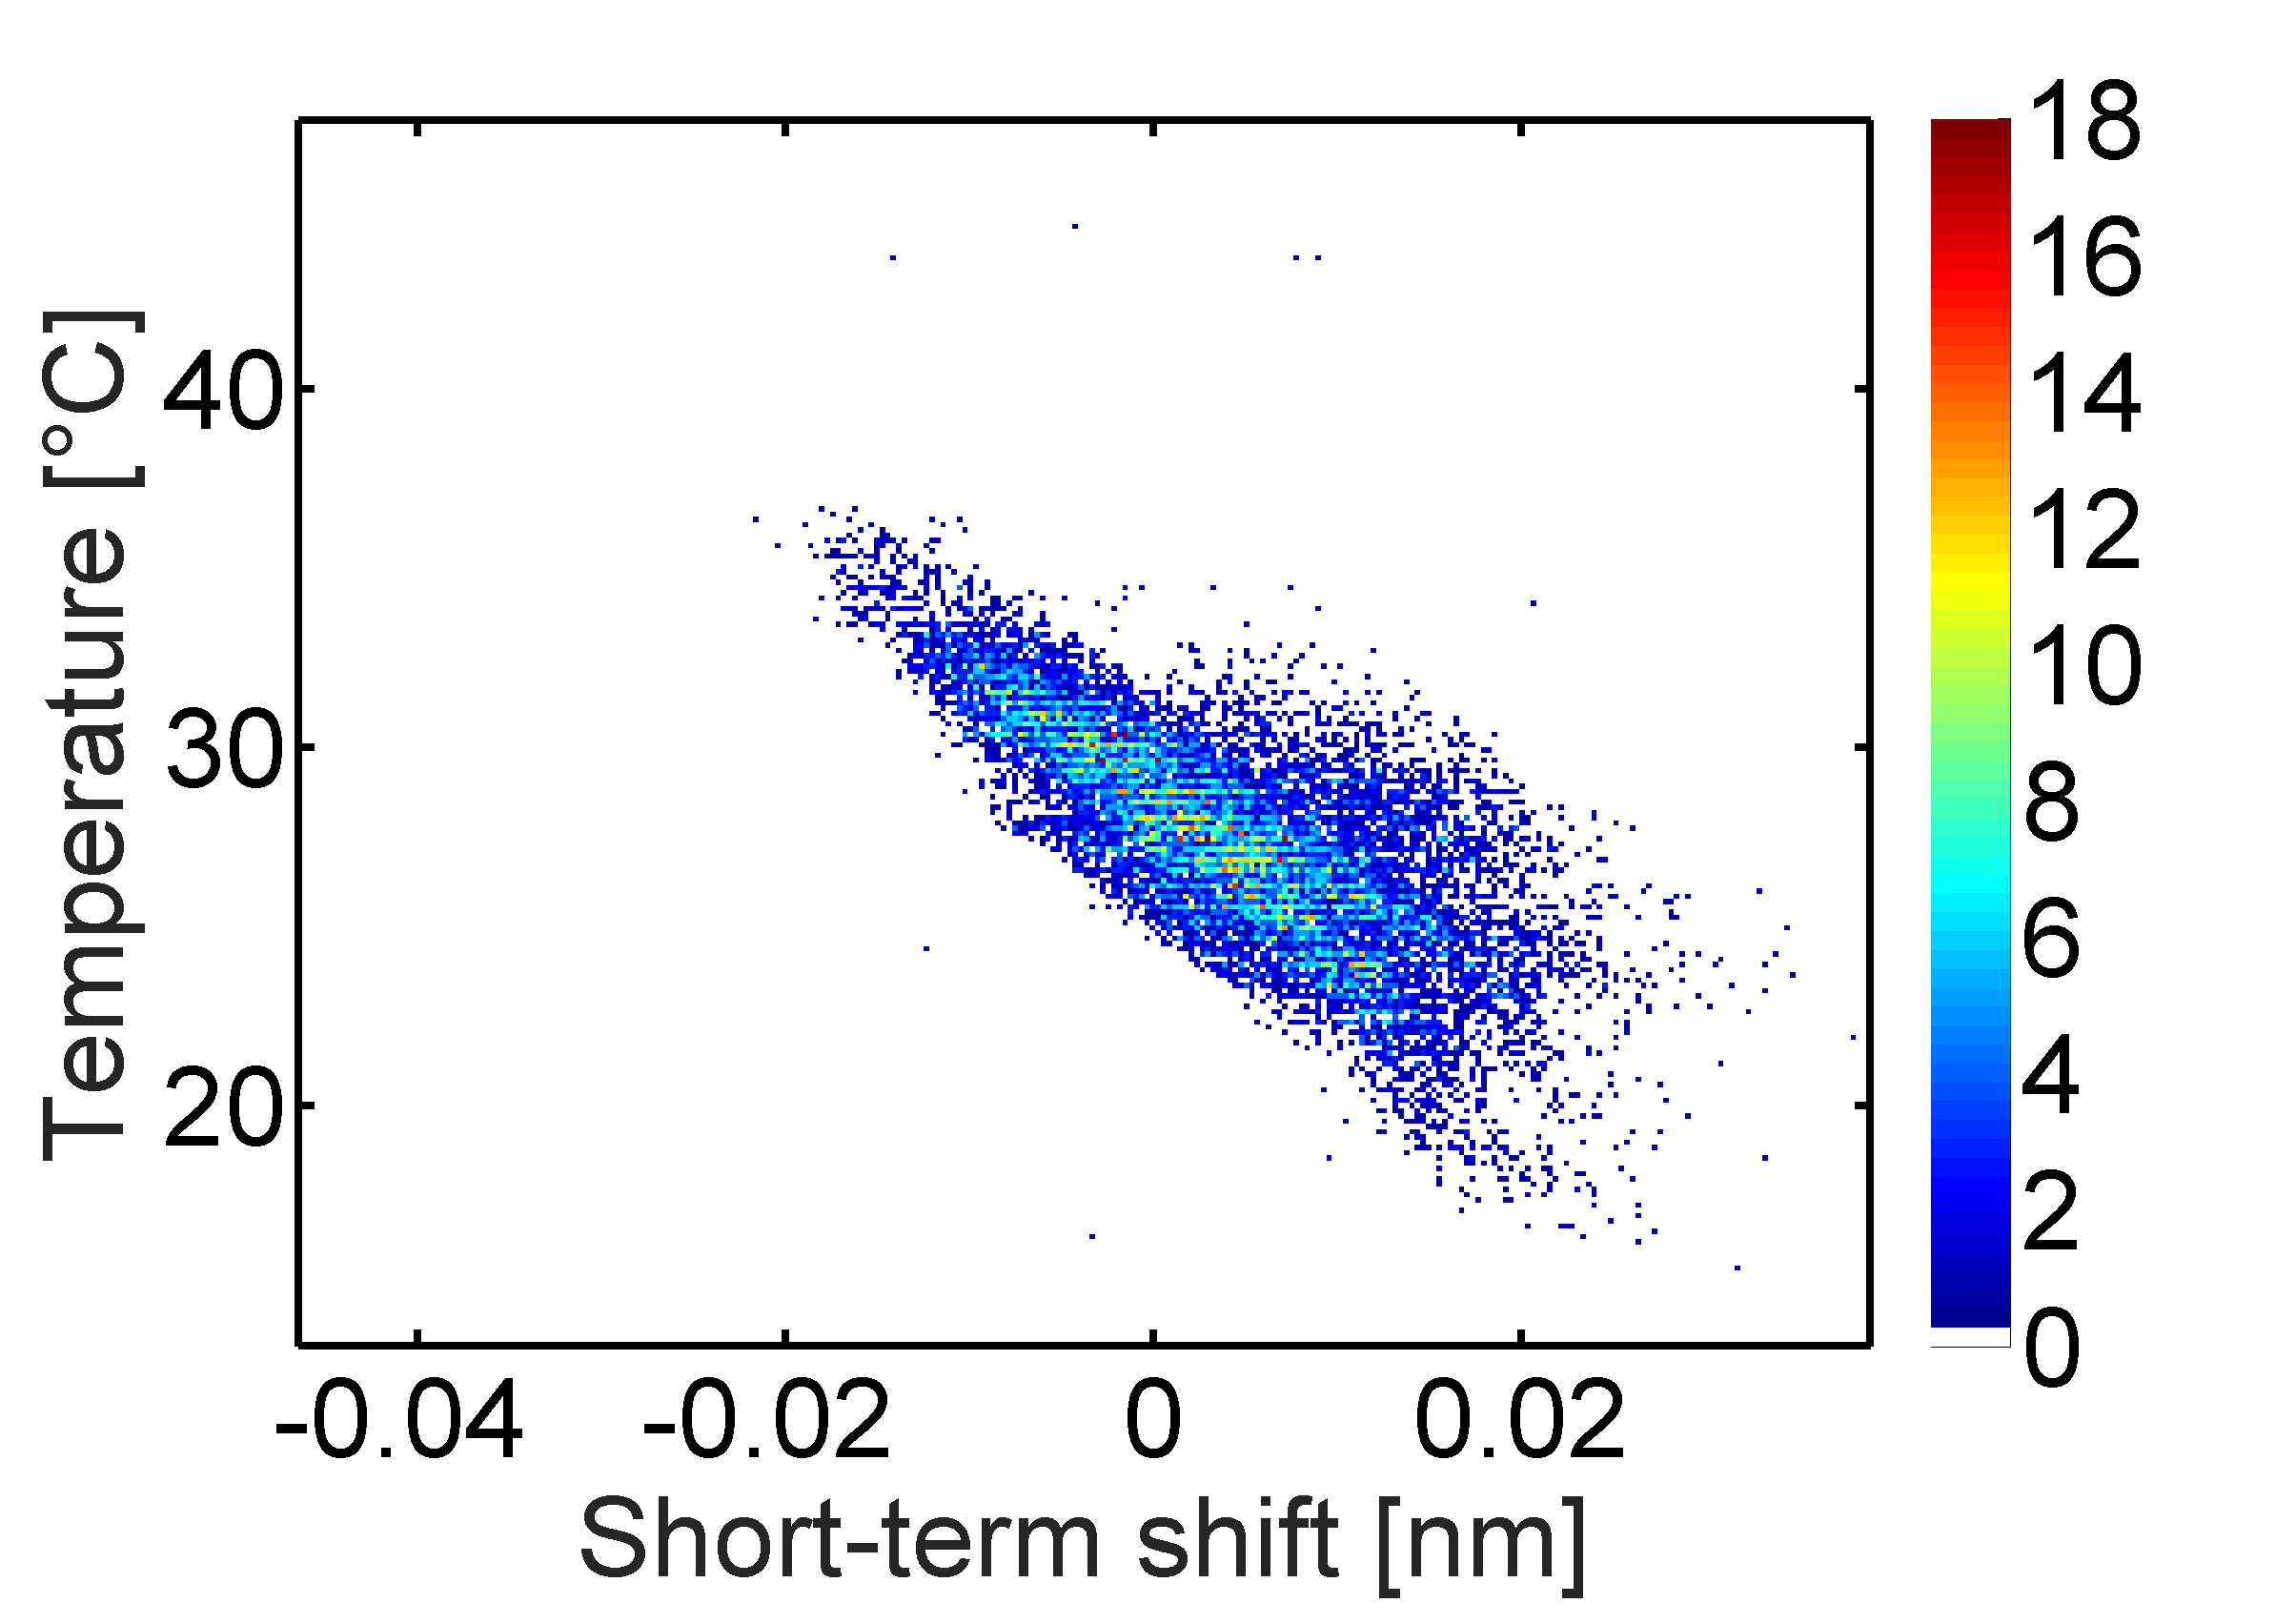
\includegraphics[width=0.49\textwidth]{Bilder/Simon/Bilder_Tung/D2J2140_After}}
	\caption{Short term wavelength as a function of the instrument temperature for Pillate 1. The coloring of the scatter points indicate the temporal evolvement. (a) initial period prior to January 2010 (b) after 2010. Source: \cite{WarnachSimon}.}
	\label{fig:shorttermshift}
\end{figure}
Moreover, \cite{WarnachSimon} show that, short term shifts are related to the instrument temperature (see \Cref{fig:shorttermshift}).\\
The above discussed temperature dependence of the WMP causes a reduction of the fit quality with increasing instrument temperature difference between plume and reference. Thus, the \ce{BrO} error also increases with the temperature difference.
Compared to the other external parameters the temperate difference has the largest impact on the \ce{BrO} error.\\
\\
% fig_curves
In \Cref{fig:difftemp} the \ce{BrO} error is plotted against the temperature difference between the plume and the reference spectrum. The blue dots show the mean \ce{BrO} error at the specific temperature difference, the standard deviation is illustrated with gray error bars. The mean \ce{BrO} deviation for the sametime evaluation is additionally marked with a red point. The plots reveal a symmetry around axis with zero temperature difference.
% tab_fit CAPTION
\begin{table}[h]
	\centering
	\begin{tabular}{|p{2cm}|p{2cm}|p{2cm}|p{2cm}|p{2cm}|p{2cm}|}
		%	\toprule
		Instrument	&D2J2140&I2J8546& I2J8548&D2J2200&D2J2201\\
		\toprule
		Slope&4.10e+12 &3.93e+12 &6.50e+12 &1.24e+13&8.17e+12 \\
		\midrule
		Correlation
		& 
		0.593& 
		0.681& 
		0.910& 
		0.886& 
		0.920\\
		\midrule
		Zero point&2.58e+13&2.23e+13&1.60e+13& 1.38e+13& 9.07e+12\\
		\midrule
		$\Delta T_{2}$&6.3&5.7&2.5&1.1&1.1\\
		\bottomrule
	\end{tabular}
	\label{tab:tempe}
	\caption{The \ce{BrO} measurement error as a function of the difference of temperature between the reference and the plume is fitted with a first order polynomial for each of the individual instruments at Tungurahua and Nevado del Ruiz. This table shows the fitting parameters slope and zero point. Moreover, the correlation between the \ce{BrO} error and the absolute temperature difference is shown. For the temperature difference this correlation with an average of $0.797$ is the highest compared to the other external parameters. In the $\Delta T_{2}$ row the temperature difference for which the error doubles compared to a temperature difference of zero is shown. This is already the case for a difference of $3.3^\circ C$}
\end{table}
% tab_fit
To quantify the dependency between the \ce{BrO} error and the difference in temperature the data are fitted with a polynom of the first order. Because of the observed symmetry around zero the absolute temperature difference is used for the fit. The computed fitting parameters slope and zero point for each instrument are shown in \Cref{tab:tempe}. \\
The zero points at Tungurahua vary from 1.6$\cdot10^{13}\frac{molec}{cm^2}$ to 2.58$\cdot10^{13}\frac{molec}{cm^2}$. The variation at Nevado del Ruiz ranges from  9.07$\cdot10^{12}\frac{molec}{cm^2}$ to 1.38$\cdot10^{13}\frac{molec}{cm^2}$.\\
Also the correlation between the \ce{BrO} error and the absolute temperature difference is shown. Here the correlation is calculated using the python library Numpy. The correlation ranges from 0.593 for the instrument D2J2140 to  0.92 for D2J2201 and exhibits a large variation between the instruments.\\
The $\Delta T_{2}$ row in the table shows the temperature difference for which the error doubles compared to a temperature difference of zero.
% tab_ratio CAPTION
\begin{table}
	\centering
	\begin{tabular}{|p{1.8cm}|p{2.15cm}|p{2.15cm}|p{2.15cm}|p{2.15cm}|p{2.15cm}|}
		%	\toprule
		Instrument	&D2J2140&I2J8546& I2J8548&D2J2200&D2J2201\\
		\toprule
		Mean&
		39.6/46.8\%&
		119.3/72.9\%
		&158.2/72.9\%
		&233.6/82.3\%
		&151.6/67.2\%\\
		\midrule
		Std&
		24.7/68.9\%&
		50.4/168.6\%&
		76.0/117.2\%&
		84.5/121.6\%&
		72.6/176.2\%\\
		\midrule
		Min&
		1/12.5\%
		&8/7.1\%&
		12/12.4\%&
		3/4.7\% &
		6/9.5\%\\
		\midrule
		Max
		&
		130	/76.9\%&
		213	/99.5\%&
		386/96.7\%&
		414	/95.6\% &
		296	/99.7\%\\
		\bottomrule
	\end{tabular}
	\caption{This table shows the absolute amount and the ratio (to \Cref{Tab:refstime}) of remaining references if restricting the temperature difference to the mean $\Delta T_{2}$ over all instruments ($Mean(\Delta T_{2}) = 3.3^{\circ}C$). Here in the ”Mean” and “Std” row for each  instrument the average restriction is shown with the corresponding standard deviation. The “Min” and “Max” rows show the extend of restriction in the extreme cases (minimum and maximum amount of available references / restriction ratio).}
	\label{tab:decTemp}
\end{table}	
% tab_ratio
If restricting the temperature difference to the mean $\Delta T_{2}$ over all instruments ($Mean(\Delta T_{2}) = 3.3$) the amount of possible references decrease as shown in \Cref{tab:decTemp}. Excluding references with temperature differences above $Mean(\Delta T_{2}) = 3.3$ restricts the amount of potential references to $46.8\%$ for D2J2140 to $82.3\%$ for $D2J2200$.\\
The advantage of restricting the accepted temperature difference is a better control of the choice of the best reference. The disadvantage is that the amount of possible references decreases. Thus, it could occur that a reference is dismissed, which has a large temperature difference but is very similar in the remaining parameters.\\

\subsection{ Daytime \label{chap:daytime}}
	\begin{figure}
	\centering
	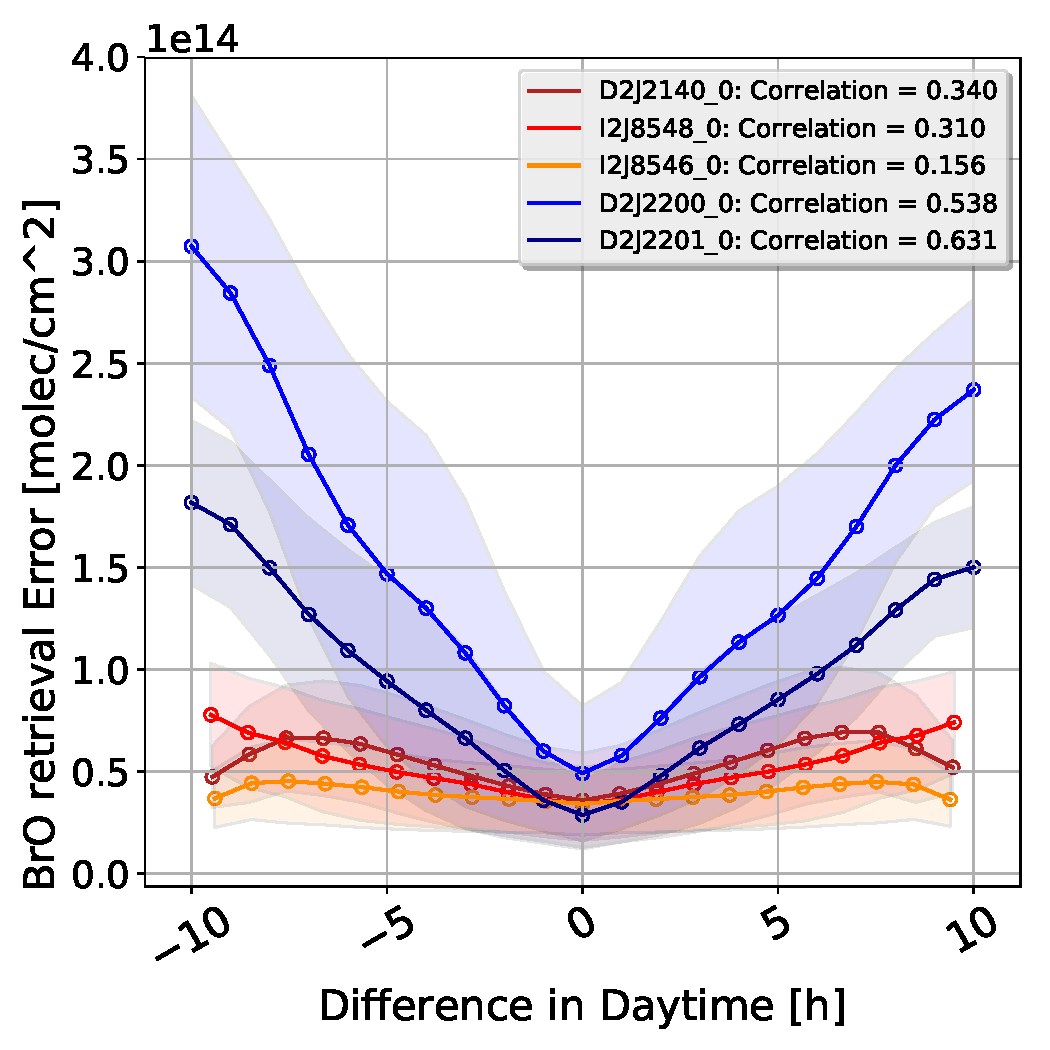
\includegraphics[width=0.7\linewidth]{Bilder/DiffDaytimeallInstruments}
	\caption{The \ce{BrO} measurement error as a function of the difference of daytime between the reference and the plume is shown for each of the individual instruments at Tungurahua and Nevado del Ruiz. To evaluate the plume spectra all reference spectra with a temporal distance of no longer than two weeks are used. An increase of the \ce{BrO} error with the absolute difference in daytime is observable. This is quantified by a correlation between the \ce{BrO} retrieval error and the absolute difference in daytime. The plots reveal a symmetry around axis with zero daytime difference. }
	\label{fig:diffdaytime}
\end{figure}
% individual text
During the day a lot of external parameters like temperature, solar altitude etc. change. In particular, the solar altitude could have an impact on the fit quality since the light path of the sun is much longer in the morning or evening compared to the noon. Therefore, the scattering effects and the Fraunehofer structures are different for both spectra.\\

% fig_curves
In \Cref{fig:diffdaytime} the \ce{BrO} error is plotted against the daytime difference between the plume and the reference spectrum. The plots are similar to the plots for the temperature: The blue dots show the mean \ce{BrO} error at the specific daytime difference, the standard deviation is illustrated with gray error bars. The mean \ce{BrO} deviation for the sametime evaluation is additionally marked with a red point. \\
As for the temperature the plots reveal a symmetry around the axis of zero daytime difference.\\
%
% tab_fit
To quantify the dependency between the \ce{BrO} error and the difference in daytime the data are fitted with a polynom of the first order. Because of the observed symmetry around zero the absolute daytime difference is used for the fit. The computed fitting parameters slope and zero point for each instrument are shown in \Cref{tab:dtcalc}. \\
%
As it can be seen in \Cref{tab:dtcalc}, the zero points at Tungurahua vary from 3.28$\cdot10^{13}\frac{molec}{cm^2}$ to 3.43$\cdot10^{13}\frac{molec}{cm^2}$. The variation at Nevado del Ruiz ranges from  2.24$\cdot10^{13}\frac{molec}{cm^2}$ to 4.01$\cdot10^{13}\frac{molec}{cm^2}$. \\
The correlations ranges from 0.156 for the instrument I2J8546 to  0.631 for D2J2201 and exhibits a large variation between the instruments.\\
The $\Delta DT_{2}$ row in the table shows the daytime difference for which the error doubles compared to a daytime difference of zero.
% tab_fit CAPTION
	\begin{table}[h]
	\centering
	\begin{tabular}{|p{2cm}|p{2.15cm}|p{2.15cm}|p{2.15cm}|p{2.15cm}|p{2.15cm}|}
		%	\toprule
		Instrument	&D2J2140&I2J8546& I2J8548&D2J2200&D2J2201\\
		\toprule
		Slope&5.07e+12&1.40e+12 &3.77e+12 &2.04e+13& 1.38e+13\\
		\midrule
		Correlation&
		0.340&
		0.156&
		0.310&
		0.538&
		0.631\\
		\midrule
		Zero point& 3.43e+13&3.39e+13&3.28e+13&  4.01e+13&  2.24e+13\\
		\midrule
		$\Delta DT_{2}$&6.8&24.2&8.7&1.9&1.62\\
		\bottomrule
	\end{tabular}
	\label{tab:dtcalc}
	\caption{The \ce{BrO} measurement error as a function of the difference of daytime between the reference and the plume is fitted with a first order polynomial for each of the individual instruments at Tungurahua and Nevado del Ruiz. This table shows the fitting parameters slope and zero point. Moreover, the correlation between the \ce{BrO} error and the absolute daytime difference is shown. In the $\Delta DT_{2}$ row the daytime difference for which the error doubles compared to a daytime difference of zero is shown.}
\end{table}

% tab_ratio CAPTION
	\begin{table}
	\centering
		\begin{tabular}{|p{1.8cm}|p{2.15cm}|p{2.15cm}|p{2.15cm}|p{2.15cm}|p{2.15cm}|}
		%	\toprule
		Instrument	&D2J2140&I2J8546& I2J8548&D2J2200&D2J2201\\
		\toprule
		Mean&
		72.0/85.1\% &		147.4/90.0\%&
		198.4/91.4\%&		275.0/96.8\%&
		205.8/91.2\%\\
		\midrule
		Std&		31.87/89.0\%&32.0/107.0\%&
		71.0/109.5\%&		70.8/101.8\%&
		50.1/121.6\% \\
		\midrule
		Min&
		6/75.0\%&		58/51.3\%
		&91/93.8\%		&54/84.4\%
		&45/71.4\%\\
		\midrule
		Max&
		160/94.7\% &
		214/100\% &
		399/100\% &
		433/100\% &
		297/100\% \\
		\bottomrule
	\end{tabular}
	\caption{This table shows the absolute amount and the ratio (to \Cref{Tab:refstime}) of remaining references if restricting the daytime difference to the mean $\Delta DT_{2}$ over all instruments except I2J8546 due to the large uncertainty ($Mean(\Delta DT_{2}) = 4.75h$). Here in the ”Mean” and “Std” row for each  instrument the average restriction is shown with the corresponding standard deviation. The “Min” and “Max” rows show the extend of restriction in the extreme cases (minimum and maximum amount of available references / restriction ratio).}
	\label{tab:daytimerest}
\end{table}	
% tab_ratio
If restricting the daytime difference to the mean $\Delta T_{2}$ over all instruments with significant impact of the daytime, ($Mean(\Delta DT_{2}) = 4.75h$) the amount of possible references decrease as shown in \Cref{tab:daytimerest}.The mean ($Mean(\Delta DT_{2})$) is calculated without taking the I2J8546 into account due to the low correlation of 0.156. Using the I2J8546 instrument as well would lead to an  $Mean(\Delta DT_{2})$ of $8.6h$, thus, the restriction would not have any influence, since the maximal time difference is limited to the time where the sun is shining.\\ 
Excluding references with daytime differences above $4.75h$ restricts the amount of potential references to $85.1\%$ for D2J2140 to $96.8\%$ for $ D2J2200$. In extreme cases a restriction down to $51.3\%$ of the entire set of references can occur.
	
\subsection{ Colorindex}
	\begin{figure}
	\centering
	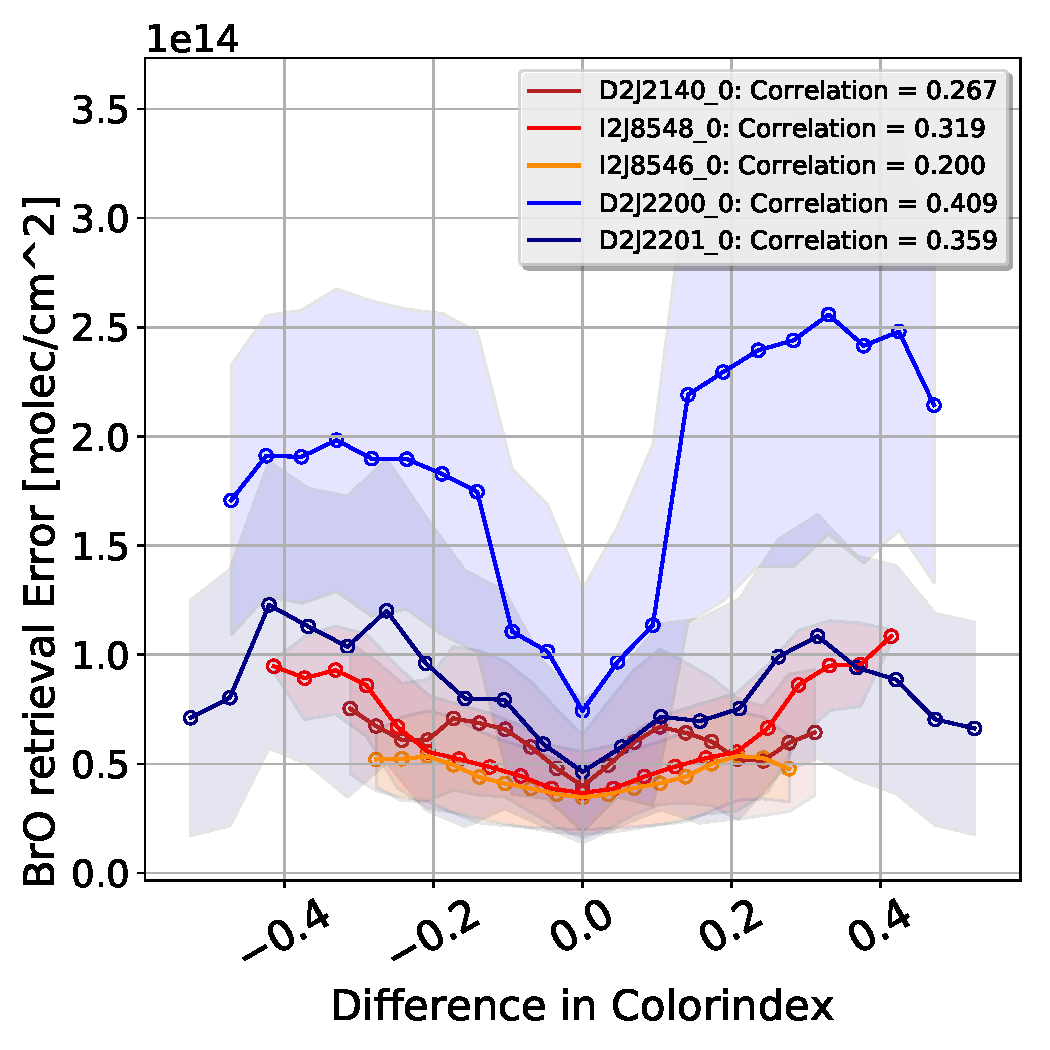
\includegraphics[width=0.7\linewidth]{Bilder/DiffColidxallInstruments}
	\caption{The \ce{BrO} measurement error as a function of the difference of colorindex between the reference and the plume is shown for each of the individual instruments at Tungurahua and Nevado del Ruiz. To evaluate the plume spectra all reference spectra with a temporal distance of no longer than two weeks are used. An increase of the \ce{BrO} error with the absolute difference in colorindex is observable. This is quantified by a correlation between the \ce{BrO} retrieval error and the absolute difference in colorindex. The plots reveal a symmetry around axis with zero colorindex difference. }
	\label{fig:diffcolidx}
\end{figure}
% individual text
Clouds  have  a  strong  influence  on  the  atmospheric  radiative  transfer  and  thus  affect  the  interpretation  and  analysis of DOAS \citep{wagner2014cloud}.
Clouds can be identified by several measurement quantities that they influence.
As Mie scattering is dominant in clouds the wavelength of the light that is scattered is different than the Rayleigh sky. Thus, clouds can be easily identified by their white color.
Therefore, the cloudiness of the sky can be quantified in a scalar measure defined by the ratio of the measured intensity at two wavelengths, the so-called colour index.
\cite{wagner2014cloud} showed that for a zenith-looking instrument the measured radiation intensity is enhanced by clouds. Thus, clouds can cause large errors for the retrieved gas column density and the corresponding uncertainties. 
Cloud effects are especially severe if the cloudiness for the recorded plume and reference spectra strongly defer. Also for broken clouds the described effect can be observed as measurements at some elevation angles might be influenced by clouds while others are not.
In this work the Colour Index (CI) is the ratio between the intensities at 320nm and 360 nm.
These two wavelengths are as far apart as the filter used for stray-light prevention in the spectrometers allows.
%% I don’t understand 	
On the other hand, the lower wavelength avoids the deep UV range where \ce{SO2} and  \ce{O3} absorption plays a dominant role.
%% I don’t understand 	
The Mie scattering in the clouds is responsible for the higher amount of radiation from larger wavelengths. This results in a decrease of the CI \citep{lubcke2014optical}.\\
We evaluated the CI at the zenith. To increase the stability of the fit we add 10 intensities. Using always the zenith to evaluate the colour index makes the colour index more comparable, but if broken clouds occur, the CI of the reference and the plume could differ from the calculated CI of the zenith. This could be a reason for the large deviations of the mean \ce{BrO} error as function of the colour index (see \Cref{fig:diffcolidx})\\
% fig_curves
In \Cref{fig:diffcolidx} the \ce{BrO} error is plotted against the colorindex difference between the plume and the reference spectrum. The plot is done similar to the plots for the temperature.
The plots mostly reveal a symmetry around the zero colorindex difference-axis. Thus, the absolute colorindex can be used for the fitting which is done equivalently to the analysis of the temperature and the daytime. The computed fitting parameters slope and zero point for each instrument are shown in \cref{tab:colidxcalc}. \\
The zero points at Tungurahua vary from 3.36$\cdot10^{13}\frac{molec}{cm^2}$ to 4.01$\cdot10^{13}\frac{molec}{cm^2}$. The variation at Nevado del Ruiz ranges from  4.74$\cdot10^{13}\frac{molec}{cm^2}$ to 7.21$\cdot10^{13}\frac{molec}{cm^2}$.\\
The correlation is as well calculated and ranges from 0.2 for the instrument I2J8546 to  0.409 for D2J2200.\\
The $\Delta CI_{2}$ row in the table shows the colorindex difference for which the error doubles compared to a colorindex difference of zero.
	\begin{table}[h]
	\centering
	\begin{tabular}{|p{2cm}|p{2cm}|p{2cm}|p{2cm}|p{2cm}|p{2cm}|}
		%	\toprule
		Instrument	&D2J2140&I2J8546& I2J8548&D2J2200&D2J2201\\
		\toprule
		Slope&2.30e+14 &7.92e+13 &1.17e+14 &5.42e+14&1.91e+14\\
		\midrule
		Correlation&
		0.267&
		0.200&
		0.319&
		0.409&
		0.359\\
		\midrule
		Zero point&4.01e+13&3.36e+13&3.47e+13& 7.21e+13& 4.74e+13\\
		\midrule
		$\Delta CI_{2}$&0.174&0.424&0.297&0.133&0.248\\
		\bottomrule
	\end{tabular}
	\caption{The \ce{BrO} measurement error as a function of the difference of colorindex between the reference and the plume is fitted with a first order polynomial for each of the individual instruments at Tungurahua and Nevado del Ruiz. This table shows the fitting parameters slope and zero point. Moreover, the correlation between the \ce{BrO} error and the absolute colorindex difference is shown. In the $\Delta CI_{2}$ row the colorindex difference for which the error doubles compared to a colorindex difference of zero is shown.}
	\label{tab:colidxcalc}
\end{table}

% tab_fit CAPTION
	\begin{table}[h]
	\centering
	\begin{tabular}{|p{1.8cm}|p{2.15cm}|p{2.15cm}|p{2.15cm}|p{2.15cm}|p{2.15cm}|}
		% 	\toprule
		Instrument	&D2J2140&I2J8546& I2J8548&D2J2200&D2J2201\\
		\toprule
		Mean&
		84.6/100\% &	163.7/100\%&	215.6/99.3\%&
		275.4/97.0\% &219.4/97.3\% \\
		\midrule
		Std&
		35.8/100\% &	29.9/100\% &
		65.4/101\%&
		67.8/97.6\% &
		49.86/121\% \\
		\midrule
		Min&
		8/100\% &
		113/100\% 
		&97/100\% 
		&61/95.3\% 
		&28	/44.4\% \\
		\midrule
		Max
		&169/100\% 
		&214/100\% 
		&399/100\% 
		&421/97.2\% 
		&297/100\%  \\
		\bottomrule
	\end{tabular}
	\caption{This table shows the absolute amount and the ratio  (to \Cref{Tab:refstime}) of remaining references if restricting the colorindex difference to the mean $\Delta CI_{2}$ over all instruments ($Mean(\Delta CI_{2}) = 0.2553.$). Here in the ”Mean” and “Std” row for each  instrument the average restriction is shown with the corresponding standard deviation. The “Min” and “Max” rows show the extend of restriction in the extreme cases (minimum and maximum amount of available references / restriction ratio).}
	\label{tab:colidxres}
\end{table}	
% tab_ratio CAPTION
% tab_ratio
If restricting the colorindex difference to the mean $Mean(\Delta CI_{2}) = 0.255$ over all instruments the amount of possible references decrease very little as can be seen in \Cref{tab:colidxres}.\\

%\begin{table}
%	\centering
%	\begin{tabular}{|p{1.8cm}|p{2.15cm}|p{2.15cm}|p{2.15cm}|p{2.15cm}|p{2.15cm}|}
%		%	\toprule
%		Instrument	&D2J2140&I2J8546& I2J8548&D2J2200&D2J2201\\
%		\toprule
%		Mean&38.98&113.8&153.2&223.8&149.37\\
%		\midrule
%		Std&
%		24.47&
%		50.6&
%		76.78&
%		82.5&
%		72.41\\
%		\midrule
%		Min&1&8&12&3 &6\\
%		\midrule
%		Max&130&213&386&399 &296\\
%		\bottomrule
%	\end{tabular}
%	\caption{Amount of potential references when restricting the external parameters as discussed above. Here the difference in CI is restricted to $0.2553$, the maximal colourindex difference is $3.358^\circ$,\textcolor{red}{besser}}
%\end{table}	

\subsection{Elevation Angle}

% fig_curves CAPTION
\begin{figure}
	\centering
	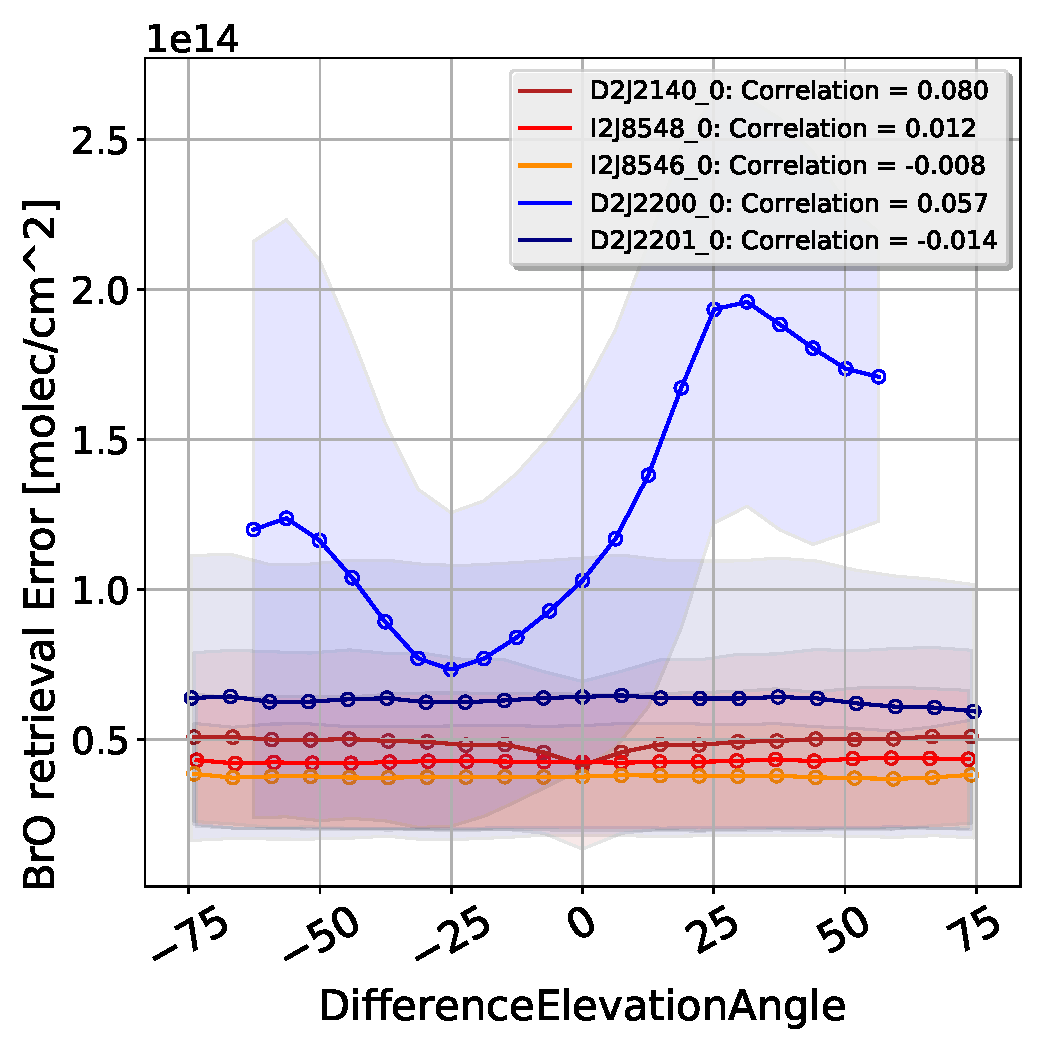
\includegraphics[width=0.7\linewidth]{Bilder/DiffElevAngleallInstruments}
	\caption{The \ce{BrO} measurement error as a function of the difference of elevation angle between the reference and the plume is shown for each of the individual instruments at Tungurahua and Nevado del Ruiz. To evaluate the plume spectra all reference spectra with a temporal distance of no longer than two weeks are used. The plots do not reveal a symmetry around axis with zero elevation angle difference for all instruments. The D2J2200 instrument at Nevado del Ruiz is not symmetric around zero.}
	\label{fig:diffeleangle}
\end{figure}
% tab_fit CAPTION
\begin{table}[h]
	\centering
	\begin{tabular}{|p{2cm}|p{2cm}|p{2cm}|p{2cm}|p{2cm}|p{2cm}|}
		%	\toprule
		Instrument	&D2J2140&I2J8546& I2J8548&D2J2200&D2J2201\\
		\toprule
		Slope& 1.73e+8& 1.55e+10  &-9.00e+9 &2.92e+11&-3.96e+10\\
		\midrule
		Correlation&
		0.000&
		-0.010&
		0.012&
		0.065&
		-0.034\\
		\midrule
		Zero point&4.77e+13&4.23e+13&3.78e+13&8.37e+13 &6.44e+13 \\
		\bottomrule
	\end{tabular}
	\caption{The \ce{BrO} measurement error as a function of the difference of elevation angle between the reference and the plume is fitted with a first order polynomial for each of the individual instruments at Tungurahua and Nevado del Ruiz. This table shows the fitting parameters slope and zero point. Moreover, the correlation between the \ce{BrO} error and the absolute elevation angle difference is shown. }
\end{table}
% same daytime / temperature plot 
%\begin{figure}
%	\subfigure{
%		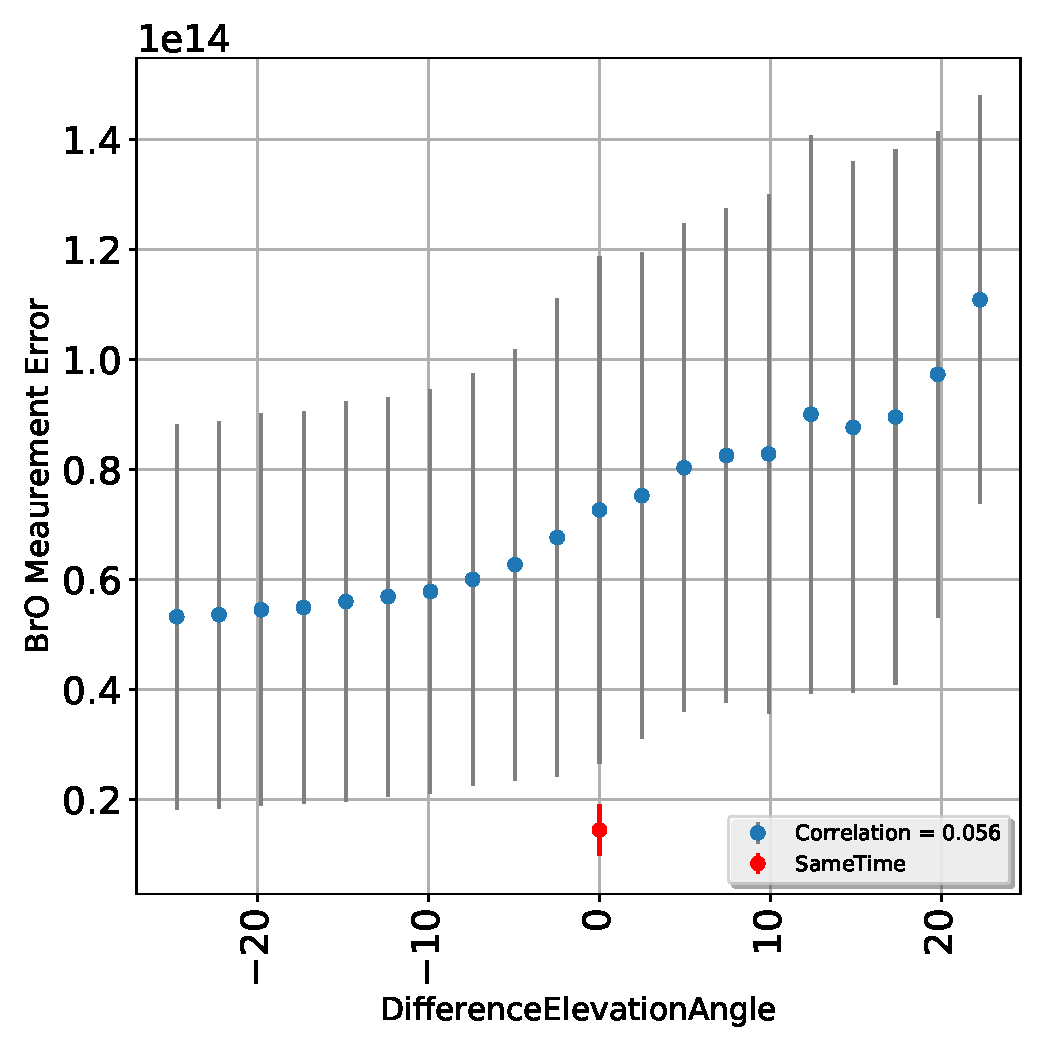
\includegraphics[width=0.49\linewidth]{Bilder/D2J2200_0_DiffElevAngle_onedaytime_Nevad}}
%	\subfigure{
%		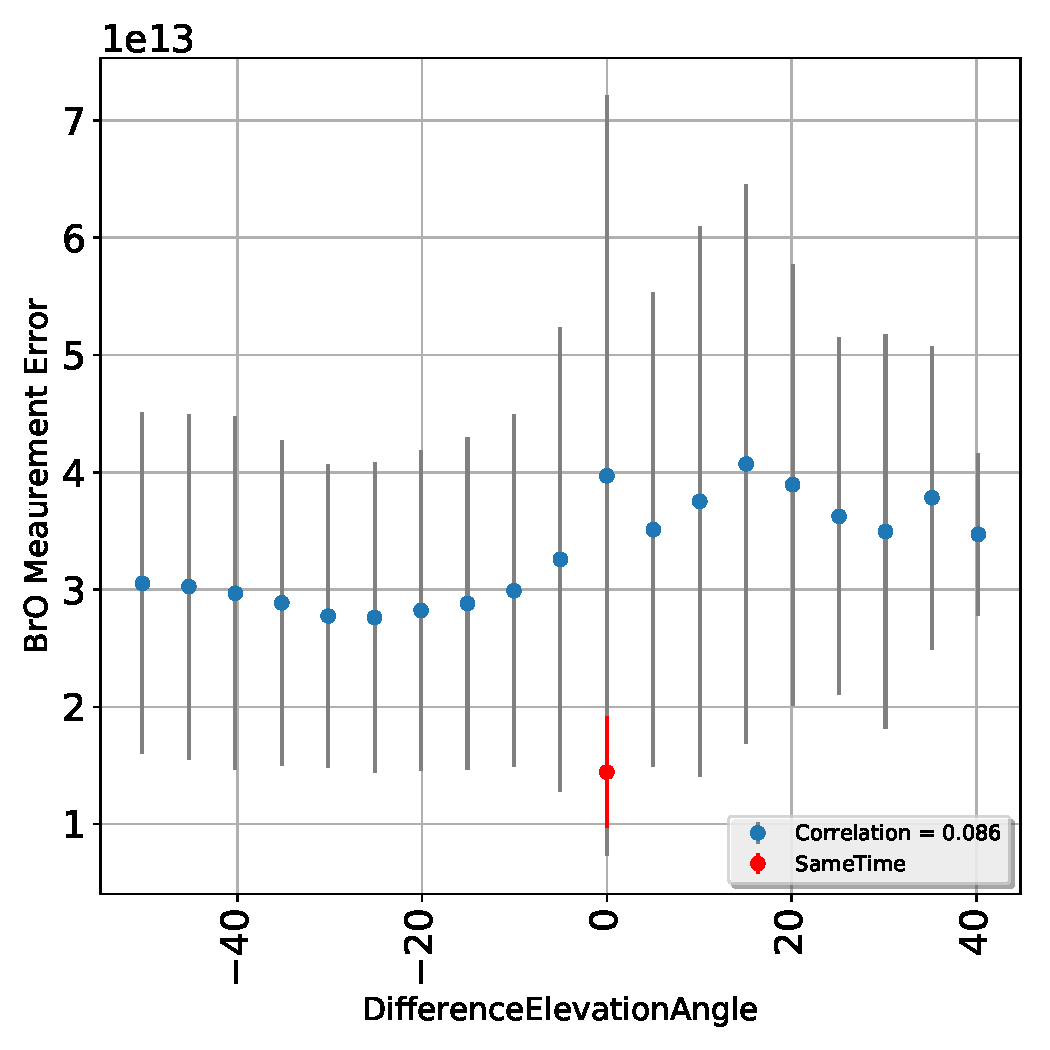
\includegraphics[width=0.49\linewidth]{Bilder/D2J2200_0_DiffElevAngle_onetemp_Nevad}}
%	\caption{The BrO measurement error as a function of the difference of elevation angle between the reference and the plumefor the D2J2200 instrument. Left: restricted to a constant difference in daytime (difference of $\pm 1h$), right: restricted to a constant difference in temperature (difference of $\pm 1^\circ$C).}
%	\label{fig:d2j22000diffelevangleonetempnevad}
%\end{figure}
\begin{figure}
	\centering
	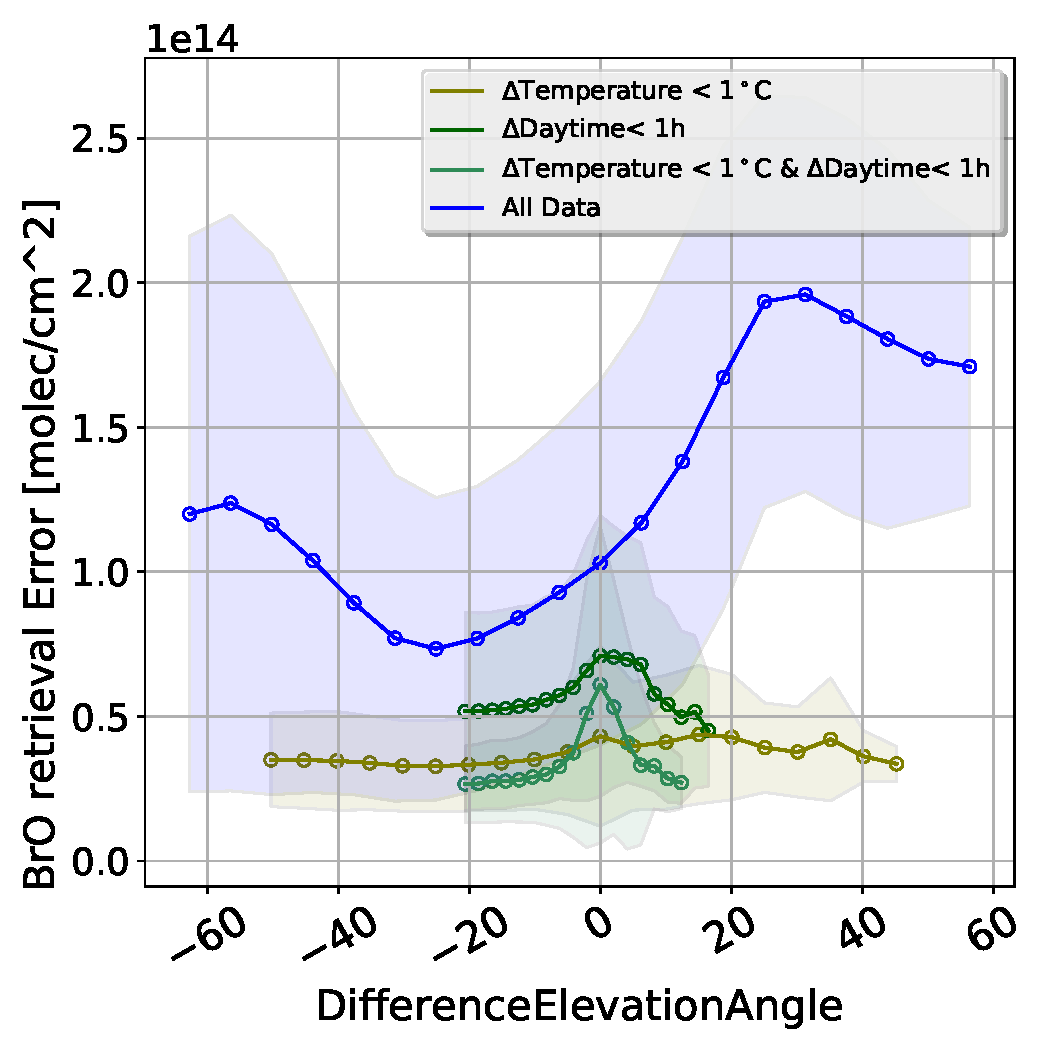
\includegraphics[width=0.7\linewidth]{Bilder/DiffElevAngleKomischesInstr}
	\caption{The \ce{BrO} measurement error as a function of the difference of elevation angle between the reference and the plume for the D2J2200 instrument. To evaluate the origin of the behavior of the \ce{BrO} retrieval error of the D2J2200 instrument as a function of the difference in elevation angle, the data are analysed on its temperature and daytime dependence. The same dependence is shown with restriction to an difference in temperature ($\Delta$Temperature) of below 1$^{\circ}C$ or restriction on a daytime difference of below 1h ($\Delta Daytime \pm 1h$). The curves are marked with different green color tones, as it is shown in the legend. The blue line shows the \ce{BrO} error as function of the elevation angle, when using all data for comprehension.}
	\label{fig:d2j22000diffelevangleonetempnevad}
\end{figure}


The elevation angle describes the angle between the horizon and the zenith. When using the plume spectrum and the reference spectrum of the same time, the difference in elevation angle cannot be zero, since the location of the plume does not coincidence with the location of the reference.\\
In \cref{fig:diffeleangle} the \ce{BrO} error is plotted as a function of the elevation angle. Obviously no significant correlation between the two parameters can be identified. This is not surprising because other than the previously discussed parameters we do not expect a more precise measurements for a difference of zero. 
Only the data of the D2J2200 instrument significantly varys with the elevation angle. The observable variation of the \ce{BrO} error with the elevation angle differs from the symmetric dependence of all other external parameter, the minimum \ce{BrO} error can be found at a difference in elevation angle of -20$^{\circ}$. This curve is a result of the solar altitude over the day which can be obtained if only using data of the same day time. Such a plot can be seen in \Cref{fig:d2j22000diffelevangleonetempnevad}.
\Cref{fig:d2j22000diffelevangleonetempnevad} shows the \ce{BrO} retrieval error as function of the difference elevation angle for the D2J2200 instrument at the Nevado del Ruiz volcano. The blue line is equivalent to the results which are shown in \Cref{fig:diffeleangle} for comparison. The green lines show data, with a maximal difference in temperature of 1$^{\circ}C$ or maximal difference in daytime of 1$h$. If restricting the data to just small differences in temperature or/and daytime, the dependency between the \ce{BrO} retrieval and elevation angle appears to be not significant. Whereas the maximum of the \ce{BrO} error can be found at an difference in elevation angle of zero.\\
\\	
Since the \ce{BrO} error does not depend significantly on the elevation angle no restriction on difference of the elevation angle is needed.
\subsection{Exposure time}
\begin{figure}
	\centering
	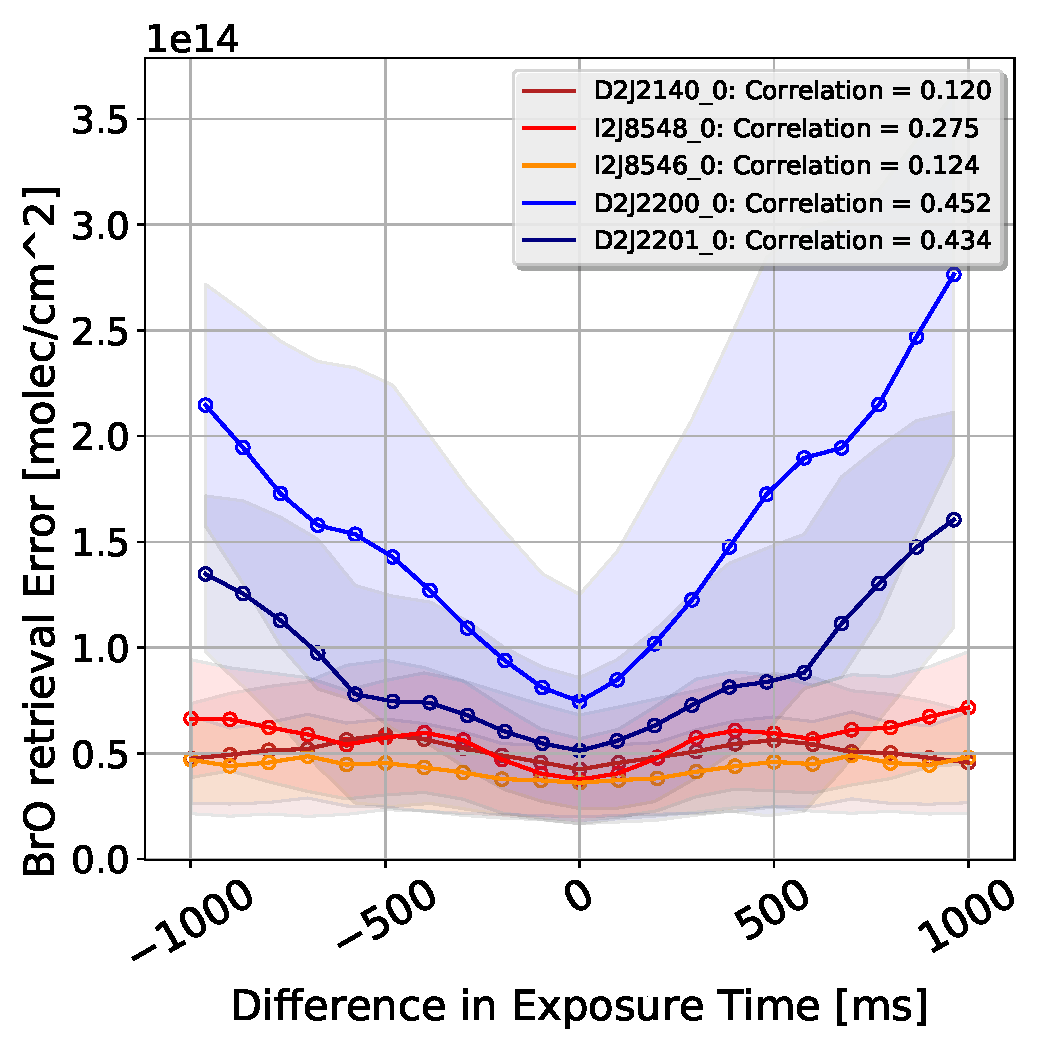
\includegraphics[width=0.7\linewidth]{Bilder/DiffExpTimeallInstruments}
	\caption{The \ce{BrO}  measurement error as a function of the difference of exposure time between measuring the reference and the plume are shown. To evaluate the plume spectra all reference spectra with a temporal distance of no longer than two weeks are used. An increase of the \ce{BrO} error with the distance in exposure time is observable.}
	\label{fig:diffexptime}
\end{figure}
The  exposure time is the length of time the sensor of the NOVAC instrument is exposed to light. In one scan the exposure time is set constant to the exposure time of the first scan, the pre reference. The amount of light that reaches the film or image sensor is proportional to the exposure time. The exposure time is adjusted in the way that the maximum intensity does not overly the capacity of the sensor. Thus, the exposure time can be used as a degree of sky lightness.\\
We can observe a small dependency of the \ce{BrO} error on the exposure time at Tungurahua and Nevado del Ruiz as it is shown in \Cref{fig:diffexptime}. The \ce{BrO}  error as a function of the difference in exposure time is also symmetric around zero for all instruments. Thus the absolute difference in the exposure time is sufficient for the evaluation.\\
The instruments at Tungurahua do not show a significant dependence (correlation coefficient between 0.067 and 0.251) on the exposure time, even though there is always a minimum of the \ce{BrO} error at a difference of the Exposure Time of 0ms.\\
Nevado del Ruiz shows a stronger correlation between the \ce{BrO}  error and the exposure time.
\begin{table}[h]
	\centering
	\begin{tabular}{|p{2cm}|p{2cm}|p{2cm}|p{2cm}|p{2cm}|p{2cm}|}
		%	\toprule
		Instrument	&D2J2140&I2J8546& I2J8548&D2J2200&D2J2201\\
		\toprule
		Slope& 5.54e+9&1.54e+10 &3.04e+10&1.72e+11&9.37e+10\\
		\midrule
		Correlation&0.067
		&0.121&
		0.251&
		0.452&
		0.434\\
		\midrule
		Zero point&4.63e+13&3.58e+13& 3.87e+13& 6.88e+13& 4.68e+13\\
		\midrule
		$\Delta T_{2}$&8357&662&1273&95&499\\
		\bottomrule
	\end{tabular}
	\caption{The \ce{BrO} measurement error as a function of the difference of exposure time between the reference and the plume is fitted with a first order polynomial for each of the individual instruments at Tungurahua and Nevado del Ruiz. This table shows the fitting parameters slope and zero point. Moreover, the correlation between the \ce{BrO} error and the absolute exposure time difference is shown.}
	\label{tab:exptimecalc}
\end{table}

\begin{table}
	\centering
	\begin{tabular}{|p{1.8cm}|p{2.15cm}|p{2.15cm}|p{2.15cm}|p{2.15cm}|p{2.15cm}|}
		%	\toprule
		Instrument	&D2J2140&I2J8546& I2J8548&D2J2200&D2J2201\\
		\toprule
		Mean&
		81.7/96.5\%		&162.8/99.4\%		&212.8/98.0\%		&284.0/100\%		&225.6/100\% \\
		\midrule
		Std&
		35.3/98.6\%&		30.1/101\%&
		64.5/99.5\% &		69.5/100\% &
		41.2/100\% \\
		\midrule
		Min  &
		8/100\%&113/100\%
		&95/97.9\%
		&64/100\%
		&63/100\%\\
		\midrule
		Max&
		167/98.8\% &
		214/100\% &
		395/99.0\% &
		433/100\%  &
		297/100\% \\
		\bottomrule
	\end{tabular}
	\caption{Amount of possible references when restricting the difference in exposure time  between plume and reference to differences below 632.25 ms.}
	\label{tab:etrest}
\end{table}	


\Cref{tab:exptimecalc} shows the slope, correlation, zero point and the $\Delta ET_{2}$s. The differences in exposure time where the \ce{BrO} error increases by a factor of two compared to the difference of exposure time of zero.
Restrictions of the exposure time to the mean of the $\Delta ET_{2}$s of all instruments which is 632.25 ms leads to an average decrease compared to \cref{Tab:refstime} of data of 98.78\%. The results for each instrument can be found in \cref{tab:etrest}.\\
\\
\\
\begin{table}
	\centering
	\begin{tabular}{|p{1.8cm}|p{2.15cm}|p{2.15cm}|p{2.15cm}|p{2.15cm}|p{2.15cm}|}
		%	\toprule
		Instrument	&D2J2140&I2J8546& I2J8548&D2J2200&D2J2201\\
		\toprule
		Mean&
		36.0/42.6\%&	112.9/69.0\%&
		148.9/68.6\%&	217.0/76.4\%&	140.4/62.2\%\\
		\midrule
		Std&
		22.35/62.4\%&
		50.6/169.2\% &
		75.9/117.1\%&
		82.1/118.1\% &
		71.0/172.3\% \\
		\midrule
		Min&
		1/12.5\%  &
		8/7.1\%  &
		12/12.4\%  &
		3/4.7\%   &
		6/9.5\%  \\
		\midrule
		Max
		&127/75.1\%
		&212/99.1\%
		&382/95.7\%
		&398/91.9\%
		&283/95.3\%\\
		\bottomrule
	\end{tabular}
	\label{tab:restrictall}
	\caption{Amount of possible references while restricting the difference in colorindex  between plume and reference to differences above 0.255. maximal Time difference is 3.358$^{\circ}C$, maximal daytime difference is 4.75h without Exposure Time  between plume and reference to differences below 632.25 ms.}
\end{table}	
\Cref{tab:restrictall} shows the amount of possible references if the only data are considered which do not exceed the thresholds in each external parameter.  The average amount of available references per plume decreases to 64\%. While the performance is as good as without the restriction, this means the averaged BrO error is almost the same (deviations are below 0.1\%).


